\documentclass[oneside,openany,obeyspaces]{book}

% ==================================== Packages ======================================
\usepackage{pdfpages}
\usepackage{listings}
\usepackage{xcolor}
\usepackage[Sonny]{fncychap}
\usepackage{etoolbox}
\usepackage{changepage}
\usepackage[
  a4paper,
  textwidth=160mm,
  textheight=250mm,
  heightrounded,
]{geometry}
\usepackage[T1]{fontenc}
\usepackage[utf8]{inputenc}
\usepackage{graphicx}
\usepackage{pgfplots}
\pgfplotsset{compat=1.18} 
\usepackage[
  backend=biber,
  style=alphabetic,
  sorting=ynt,
]{biblatex}
\addbibresource{references.bib}
\usepackage[hidelinks]{hyperref}
\usepackage{titlesec}
\usepackage{fancyhdr}
\pagestyle{fancy}
\fancyfoot[C]{\thepage} % Centered pagenumber on the bottom. ("\cfoot{\thepage}" is deprecated.)
\usepackage[skip=10pt plus1pt, indent=30pt]{parskip}
\usepackage{soul}

%New colors defined below
\definecolor{codegreen}{rgb}{0,0.6,0}
\definecolor{codegray}{rgb}{0.5,0.5,0.5}
\definecolor{codepurple}{rgb}{0.58,0,0.82}
\definecolor{backcolour}{rgb}{0.95,0.95,0.92}

%Code listing style named "mystyle"
\lstdefinestyle{mystyle}{
  backgroundcolor=\color{backcolour},   commentstyle=\color{codegreen},
  keywordstyle=\color{magenta},
  numberstyle=\tiny\color{codegray},
  stringstyle=\color{codepurple},
  basicstyle=\ttfamily\footnotesize,
  breakatwhitespace=false,         
  breaklines=true,                 
  captionpos=b,                    
  keepspaces=true,                 
  numbers=left,                    
  numbersep=5pt,                  
  showspaces=false,                
  showstringspaces=false,
  showtabs=false,                  
  tabsize=2
}
\usepackage{longtable}
% ==================================== Preamble ======================================

\setlength{\parskip}{1.2ex}        % space between paragraphs
\setlength{\parindent}{0cm}        % amount of indention
\ChTitleVar{\Huge\bfseries}


\titleformat{\chapter}[display]
  {\normalfont\filleft}{\Huge\scshape\chaptertitlename\ \thechapter\\*[0pt]\hrulefill}{-10pt}{\Huge\bfseries}[\vspace{-25pt}\hrulefill]
\titlespacing*{\chapter}
  {-10pt}{0pt}{0pt}
  
\newcommand\Tstrut{\rule{0pt}{4.6ex}}       % "top" strut
\newcommand\Bstrut{\rule[-1.9ex]{0pt}{0pt}} % "bottom" strut
\newcommand{\TBstrut}{\Tstrut\Bstrut} % top&bottom struts
\newenvironment{subs}
  {\adjustwidth{3em}{0pt}}
  {\endadjustwidth}

\definecolor{codegreen}{rgb}{0,0.6,0}
\definecolor{codegray}{rgb}{0.5,0.5,0.5}
\definecolor{codepurple}{rgb}{0.58,0,0.82}
\definecolor{backcolour}{rgb}{0.95,0.95,0.92}

\lstdefinestyle{mystyle}{
    backgroundcolor=\color{backcolour},   
    commentstyle=\color{codegreen},
    keywordstyle=\color{magenta},
    numberstyle=\tiny\color{codegray},
    stringstyle=\color{codepurple},
    basicstyle=\ttfamily\footnotesize,
    breakatwhitespace=false,         
    breaklines=true,                 
    captionpos=b,                    
    keepspaces=true,                 
    numbers=left,                    
    numbersep=5pt,                  
    showspaces=false,                
    showstringspaces=false,
    showtabs=false,                  
    tabsize=2
}

\lstset{style=mystyle}
\newcommand\tab[1][1cm]{\hspace*{#1}}
\newcommand\TeamName{Cringe Coders Team}
% ================================== Title Page ======================================

\begin{document}

\begin{titlepage}
    \begin{center}
        \vspace*{0.25cm}
        \begin{huge}
            \textsc{\textbf{Semester Project Final Report}}
        \end{huge}

        \vspace{0.5cm}

        \begin{Large}
            \textsc{\textit{Computer Science Learning Center Website Project}}\\~\\
            \textsc{\textit{\TeamName}}
        \end{Large}

        \vspace{1.5cm}

        \textsc{
            \textbf{Austin Bailey}\\
            \textbf{Mya Bell}\\
            \textbf{Lindsey Langdon}\\
            \textbf{Nolan "OG" Gregory}
        }

        \vfill

        \textsc{Semester Project Final Report for the\\
            Computer Science Learning Center Website Project\\}

        \vspace{0.8cm}

        \textsc{Dr. Harvey Siy; College IS\&T\\
            University of Nebraska - Omaha\\
            Capstone Course\\
            October 12th, 2023}\\~\\

        \textit{Report prepared in fulfillment of CSCI 4970: Computer Science Capstone Project}
    \end{center}
\end{titlepage}

\tableofcontents


% ================================== Main Content ======================================
\begin{flushleft}
    \chapter{Introduction}

    \section{Motivation} \label{sec:Motivation}

    \tab The Computer Science Learning Center (CSLC), is a student service hosted through the College of Information Science \& Technology (IS\&T) for academic assistance and tutoring. The CSLC accepts tutoring by appointment or walk-ins Monday through Saturdays, and distance tutoring over Zoom. Student-tutors are paid for their services, and the University has administrators to oversee and manage CSLC staffing levels, work shifts, and payroll.\\~\\

    \tab The existing CSLC portal has incomplete or missing features, functionality, and services. The current ticket submission system functions through a Google Form tied to a spreadsheet with the resulting student information.\\~\\

    \tab To better meet the needs of the CSLC, the \TeamName\space proposes a full stack refresh of the existing technology stack. The ticketing system at present will be rebuilt to provide tutors and students with a more efficient way for exchanging essential information. This encompasses sharing specifics about the class assistance needed, articulating the present comprehension of the problem, identifying the respective course instructor, and the level of priority. The new portal will be able to facilitate this seamless sharing of this information between tutors and students.\\~\\


    \section{Similar Applications}

    \tab Last semester's capstone course had a group lay the foundations of the project work, including a basic website with some more advanced functionality like authentication. While a CSLC tutoring portal exists, the current solution does not have the full suite of functionality that the client desires. This includes a ticketing for students to request tutoring, dynamic web page elements to show new tickets without the need to refresh the page, UI/UX considerations, and report generation for tracking ticket trends.\\~\\

    \tab Core elements of infrastructure were established with the prior group, but some supplemental features were given work-around solutions. Case and point is the ticketing and reporting functionality. The current implementation is to use Google Forms to submit tickets, which allows for a limited (alibeit incorrectly and partially formatted) report.\\~\\

    \tab In light of the limitations of current solutions, the \TeamName\space takes this as a motivation to overhaul the UI/UX and add further back-end functionality, as is highlighted in our \hyperref[sec:Motivation]{Motivation} section via a proposed solution outlined in \hyperref[chp:Architecture and Design]{Chapter 3: Architecture and Design}.\\~\\
    {\color{red}Comment 1.1: Your application type is a little harder to pin down. It is also similar to IT help desk ticketing systems like Zendesk, SolarWinds or ServiceNow. Can you look up some features from such systems? Also, it is similar to tutor tracking systems, like this one: \url{https://www.go-redrock.com/solutions/tutortrac/}\\~\\}
    {\color{blue} \tab The \TeamName's current conception of such a project would take inspiration from ticket management solutions, such as ServiceNow. ServiceNow provides ticketing for requests, incidents, and miscellaneous processes that allows an organization a central way of tracking and administrating business processes. More in line with \TeamName's focus would be a solution like \url{https://www.go-redrock.com/solutions/tutortrac/}\\~\\}

    \section{Theoretical Foundations of the Project}

    \tab The back-end database structure established by the prior group will likely need modification and updates, and thus necessitates additional modeling and design of structured tables and potentially databases (Connolly \& Begg, 2014). Additionally, the data needs to be accessible via REST API, such that Django REST can make API calls to the database, for both read and write operations (Fielding, 2000).\\~\\

    \tab Though the CSLC is labeled 'Computer Science', the CSLC services all IS\&T majors and students. Consequently, security practices should be implemented in the development and deployment of a CSLC portal. This includes protecting against common security flaws, such as Cross-Site Scriting (XSS),  and Cross-Site Request Forgery (CSRF) (OWASP, 2021). Much of this security will derive from proper implementation of front-end developments through proper project management of Django (Django Project, 2021).\\~\\


    \section{Software Engineering Challenges}

    \tab We anticipate only trivial computer science challenges will arise in the scope of work. The only challenge revolves around the synchronization of the front-end and back-end for real-time updates. Successfully establishing seamless communication between these elements, alongside the portal's relational sqllite database, is mentioned because the implementation is novel to the \TeamName.\\~\\

    \tab This in not to suggest we anticipate no challenges. The success of this project hinges on everyone's familiarity with the technology stack in use. For some team members, and potentially he entire team, this means dedicating time to become acquainted with new frameworks and programming languages. The capacity to acquire new skills is essential in the world of software engineering. Also, given that not all team members have worked together before, getting an understanding on each other's work processes presents an additional challenge. In essence, the success of this project not only hinges on the team's technical expertise but also equally relies on the team's collaboration and communication.\\~\\


    \section{System Context}

    \tab The CSLC portal will occupy the intersection of faculty and student academic interests. The current and proposed solution are designed to facilitate tutoring by, and for, IS\&T students. Below \TeamName\space outlines the various facets of the system's context.\\~\\

    \subsection{Subject Facet}

    \tab Kyle runs the CSLC, which tutors students via a ticketing system. Students request help in a certain subject or class, and the CSLC pairs them with an appropriate tutor. The CSLC is the official tutoring center for IS\&T. Kyle uses ticket history to run a periodic report, detailing the classes that students struggle with most. Tutors at the center are paid employees and they use the ticket queue to find students they're qualified to help.\\~\\

    {\color{red}Comment: 1.2: Explain the scope of topics that CSLC can help with. For example, programming assignments, maybe discrete math? Does CSLC help with database questions or environment/configuration troubleshooting? How about Git? \\~\\}

    {\color{blue}\tab The \TeamName's scope of topics include, but are not limited to, UI/UX, Database design, software engineering, and version controling via Github. We anticipate that various MIS electives and the software engineering course to be a primary source of inspiration and guidance in addressing the broader scope.}
    \subsection{Usage Facet}

    \tab The primary stakeholder is Kyle Reestman, who is the director of the Computer Science Learning Center and therefore oversees all of the operations within. The users of the system will include the students, student-tutors, teachers, and other staff members associated with the computer science department of the University of Nebraska at Omaha.\\~\\

    {\color{red}Comment 1.3: Discuss what information is usually tracked in the old system. Another aspect to describe here is the state of the students who are asking for help. Based on your experience, what are common student attitudes when they ask for help? Sometimes, when students are tired or stressed, it affects how they interact with systems. \\~\\}

    {\color{blue}\tab It is important to take note of the mental state of students who are using the portal. Most of the time that students are seeking help with school work, they are in a stressed and somewhat agitated state. This is another reason why having an easily usable interface for the tutoring portal is important. \\~\\}

    \subsection{IT System Facet}

    \tab Submitting a ticket on the CSLC Portal will be one of the first interactions a student will have with the CSLC. Therefore, it is crucial that this application will seamlessly fit into the already established technological environment. For context, the CSLC is tied to the University of Nebraska-Omaha. As a result, the reconstructed portal will have to conform with UNO's current authentication system and present a polished and professional user interface.\\~\\

    \subsection{Development Facet}

    \tab The main development concern with this portal is the familiarity with technology stack. To create a web application up to professional standards, everyone must be well-versed with the languages at hand. The team's overall proficiency with the technology stack will not only enhance the development process but also contribute to the long-term success and sustainability of the project.\\~\\

    \subsection{Legal \& Ethical Facet}

    \tab We foresee no legal requirements, as the ingestion of data is self-reported by students, and only the tutors and Kyle can see it. Since this project will not integrate with other systems, basic security and architecture protections will suffice. The only possible issue we foresee is FERPA regulations limiting the projects integrating or sharing data with other systems.\\~\\

    \tab Ethically, we believe any value-added aspects, such as ‘About Us' or mission and vision statements have been addressed by the last capstone group. Our focus ethically will be around presenting a clean and professional interface for students. We believe that a haphazard or poorly designed interface will reflect poorly on the CSLC and serve to discredit the tutors by showing poor computer science principles on the CSLC website.\\~\\

    {\color{red}Comment: 1.4: Another important ethical concern is fairness. This influences which students are helped next, and may affect how long they are being helped. Another is respect, providing a welcoming and inclusive feel, including from using the app.\\~\\}

    {\color{blue}\tab \TeamName will implement the ticketing system to holistically mirror the prior online version and the in-person experience. As such, ticketing will be on a first-come-first-serve basis, with small caveats for specialty topics or courses, that only specific tutors may be able to cover. In such circumstances, the new version will follow the principles of the old and in-person system, with advanced notice or scheduling requirements. This conforms to the clients specifications and produces an egalitarian system.}



    \chapter{Requirements}

    \section{Goals}

    \subsection{Goal Model}

    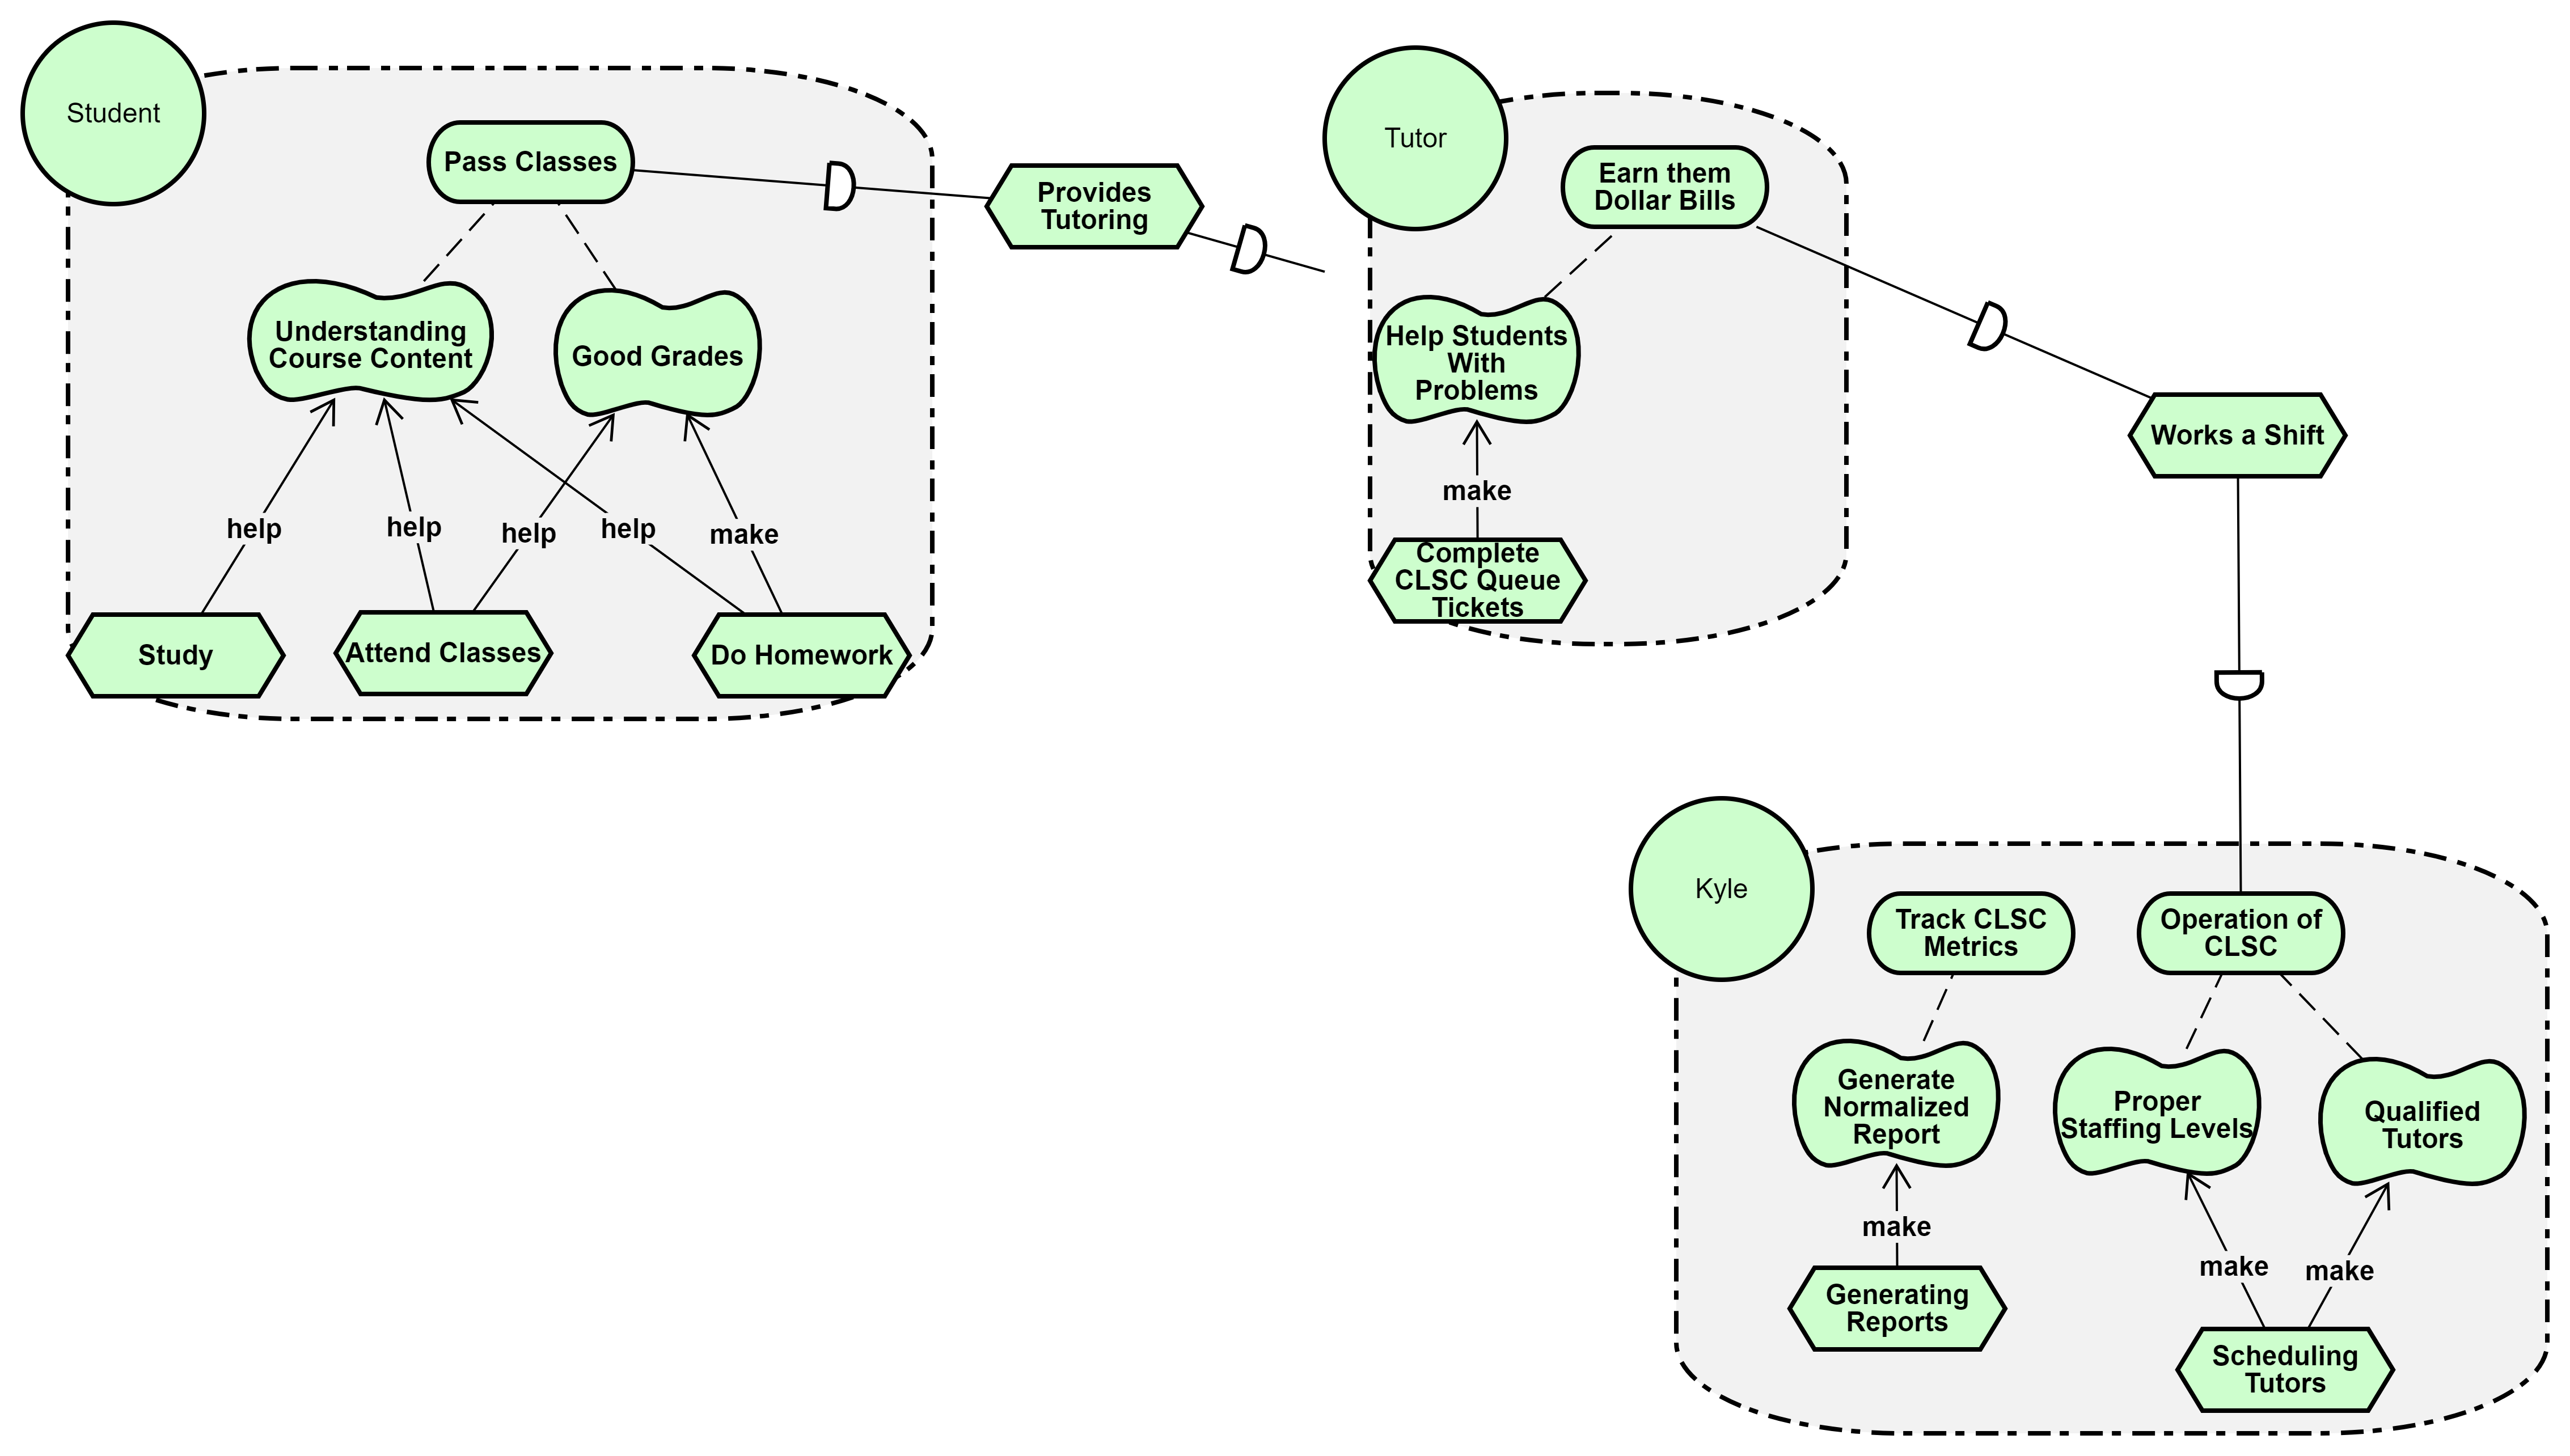
\includegraphics[width=160mm,scale=0.5]{img/goalDiagram.png}\\~\\

    \subsection{Goal Descriptions}

    \tab The Student is one of the users of the system. Each student has an overarching goal of passing their classes, which the CSLC portal is designed to aid in. Students will use the portal as a tool that will connect them with people who will help them to understand the content they need help with.\\~\\

    \tab The Tutor is employed by the CSLC to tutor students. One of the main functionalities of the CSLC portal is the ticketing system. This function makes it easy for tutors to plan and organize what they need to do.\\~\\

    \tab Kyle oversees the CSLC, so he has a goal of ensuring the smooth operation of the whole thing. The CSLC portal is designed to aid him in this goal by making it easy to schedule tutors and track what is actually going on.\\~\\


    \section{Functional Requirements} \label{sec:Functional Requirements}

    \begin{enumerate}
        \item \underline{Must have}. As the director of the Computer Science Learning Center, I want the CSLC portal to have efficient ticket management, so that tutoring requests can be managed.
        \item \underline{Must have}. As a tutor at the Computer Science Learning Center, I want to be able to interact with students and administrators regarding tutoring requests and progress as well as close and edit tickets, so that I can effectively provide help to students.
        \item \underline{Must have}. As a student I want to be able to make tutoring requests and see available tutors so that I can receive the help I need.
        \item \underline{Should have}. As an administrator, I want to be able to view and manage student requests, so that I can monitor progress and efficiency within the CSLC.
        \item \underline{Could have}. As a student, I want to be able to see how tutors are rated among other students, so that I can make an informed decision about choosing a tutor.
        \item \underline{Won't have}. As a user of the CSLC portal, I do not want to have to log in and authenticate redundantly, so that ticket submission is time efficient.
    \end{enumerate}
    {\color{red}Comment 2.1.1:	Connect the “so that” statements to goals in your goal model. This may mean adding more high level goals to the goal model.\\~\\}
    {\color{red}Comment 2.1.2:	Review these functional requirements and make sure that this section has covered all the features you actually implemented and that they behave consistently as described. Add any missing ones. In particular, User Stories \#1 and \#2 need to be expanded into multiple user stories for each feature you implemented in support of efficient ticket management and student interaction. Other additional features include querying capabilities, importing the current semester's schedule to identify instructors and courses, etc. \\~\\}
    {\color{red}Comment 2.1.3:	Move any unimplemented requirements to Section 2.8.\\~\\}
    {\color{blue}\tab Added filler to 2.8\\~\\}

    \section{Wireframes}

    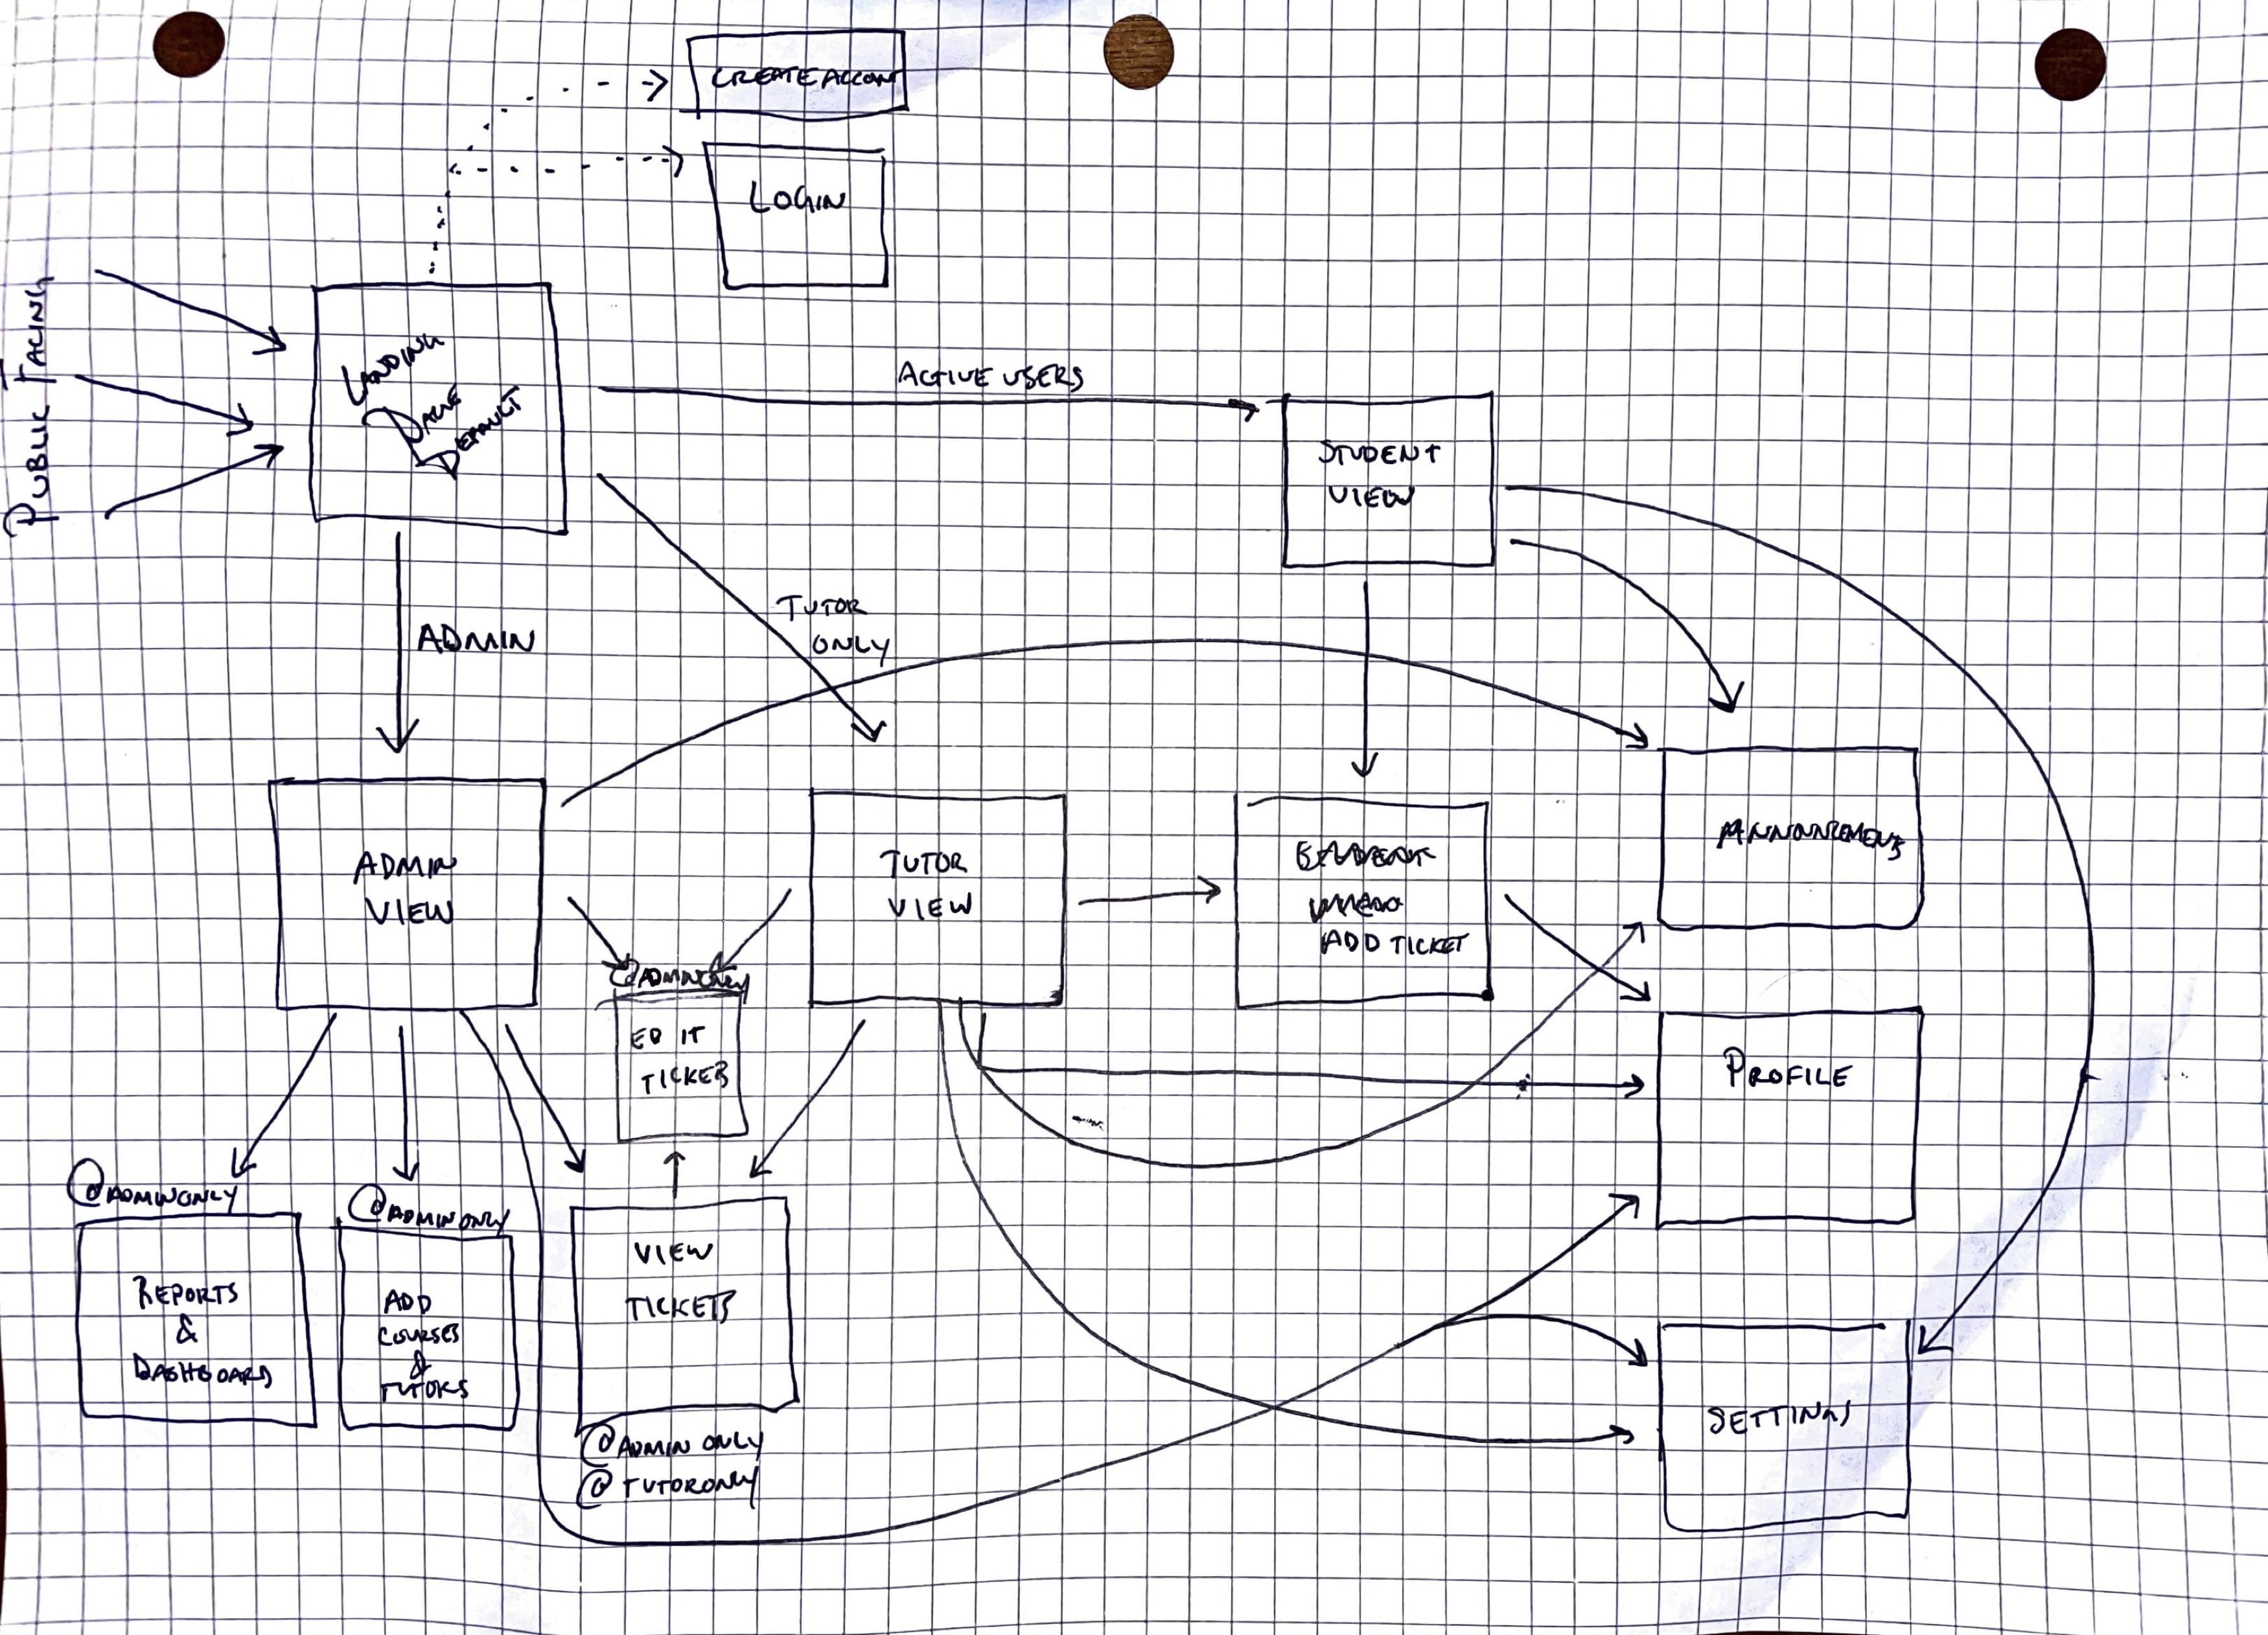
\includegraphics[width=160mm,scale=0.5]{img/wireframe.jpg}\\~\\


    \section{Object Model}

    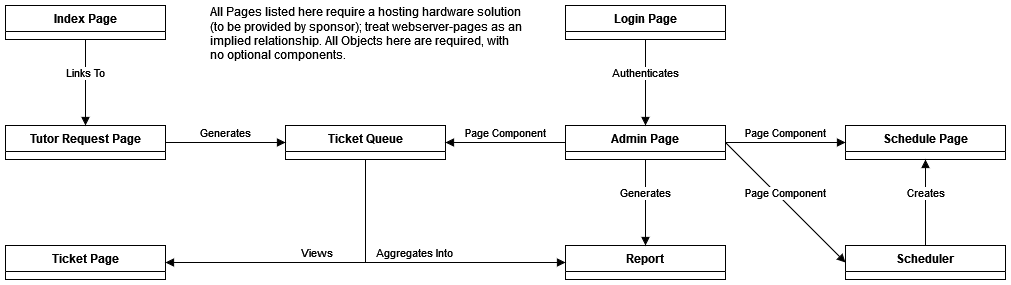
\includegraphics[width=160mm,scale=0.5]{img/UML Object Model.png}\\~\\
    {\color{red}Comment 2.2: Other objects: Ticket (which goes into Ticket Queue), Problem and Course which are referenced by Ticket, Student who submitted the Ticket.\\~\\}

    \section{Nonfunctional Requirements}

    \begin{enumerate}
        \item Must have: Evaluating the CSLC Tutoring Portal application on ease of use from the point of view of the students in the context of submitting a ticket for help.\\
              \tab Q1: How easy is it to navigate the user interface?\\
              \tab\tab M1. Task time\\
              \tab\tab M2. Stroke count\\
              \tab\tab M3. Problem count\\
              \tab Q2: How quickly can tasks be accomplished?\\
              \tab\tab Reuse M1, M2, M3\\
              \tab Q3: Do users feel satisfied after using the portal?\\
              \tab\tab M4. Conduct surveys to find the percentage of students reporting high satisfaction after using the portal\\

        \item Should have: Assess the CSLC Tutoring Portal application on maintainability from the point of view of the developers in the context of ensuring that the application is up to date.\\
              \tab Q1: How maintainable are the languages in the stack?\\
              \tab\tab M1. Check how often the languages are updated\\
              \tab Q2: How many dependencies are there?\\
              \tab\tab M2. Count the dependencies\\
    \end{enumerate}


    \section{Analysis Requirements}

    \tab \TeamName determined that we have no analysis requirements.\\~\\


    \section{External System Interfaces}

    \begin{itemize}
        \item API specifications of existing systems that interact with your product, e.g., the name of the application being accessed, services called, parameters passed, outputs returned, set up instructions (e.g., API keys)
        \item file formats your product is required to use, e.g., if you had to input from, or output to a file with a certain csv format
    \end{itemize}

    \tab (add content as needed) Microsoft SSO API? Report style?\\~\\

    \tab Attached in the appendix is a static copy of the Sphinx auto documentation that clarifies the full API interface, both internal and external. additionally, within the administrative interface, Kyle or another administrator can download a csv of the tickets table.\\~\\


    \section{Requirements Not Implemented}

    \tab \TeamName was able to quickly prototype, develop, and implement our capstone solution. Therefore, we have implemented all requirements, and were able ot address small stretch goals.\\~\\




    \chapter{Architecture and Design} \label{chp:Architecture and Design}

    \section{Overview}

    \tab The CSLC portal will comprise a handful of web pages hosted on the \url{https://cslc.unomaha.edu/} subdomain, with integration of a back-end database. at a high-level technology-agnostic view, we have the following design requirements\\~\\

    \begin{enumerate}
        \item A guest, index, or public page that links to the portals resources.
        \item A ticket or tutoring request submission resources.
        \item A tutor or employee view that allows access to the ticket queue and shift schedules of tutors.
        \item An admin view that allows the client to export reports based on ticket history, and to configure work schedules.
        \item A back-end database to facilitate the ticketing processes.\\~\\
    \end{enumerate}

    \tab Subsequent sections will cover these designs through the various lens, culminating in a more concrete description of architecture.\\~\\


    \section{Logical Decomposition View}

    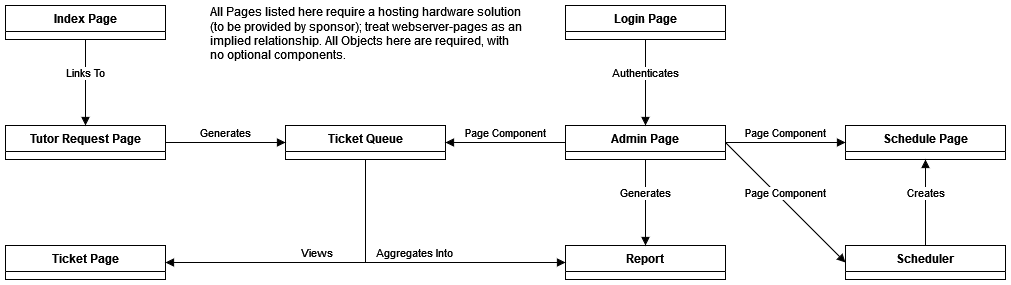
\includegraphics[width=160mm,scale=0.5]{img/UML Object Model.png}\\~\\

    \tab \TeamName provides a simplified UML diagram of both the public and administrative functions of the CSLC portal. Note that the decomposition has merged the  employee and admin pages, as the \TeamName's current intent is to implement RBAC roles associated with authenticated users that reveal components of the admin page. This will ideally minimize redundant pages and code.\\~\\

    \tab For the sake of simplicity and ease of conveying design, the database subsystem has been omitted, as it will integrate will almost every other subsystem.

    \tab to see the \TeamName's accompanying functional requirements, see the \hyperref[sec:Functional Requirements]{Functional Requirements} section.\\~\\
    {\color{red}Comment 3.1: Based on this object model, the system can be broken down into two subsystems: Ticket Management that encompasses every feature related to submitting and processing tickets, and Tutor Management which is the administrative side of the CSLC (adding and updating tutors, scheduling tutors, etc.). \\~\\}

    \section{Technology Stack}

    \tab The \TeamName\space intends to replace the current portal with a full refresh of the technology stack. Additionally, will add database tie-ins to the portal to replace the current Google Form solution.\\~\\
    {\color{red}Comment 3.2: Make sure to update this to reflect the technologies used in the final implementation. \\~\\}

    \subsection{Languages}

    \tab For this project, we used the following languages: Python, JavaScript, TypeScript, HTML, and CSS. We also had a marginal presence of the Makefile and Dockerfile languages to aid in deployment of the project. The language usage stems primarily from the  Django, React, and Tailwind frameworks and libraries.\\~\\
    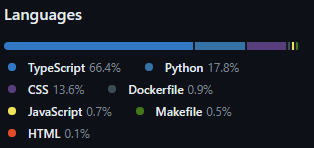
\includegraphics[width=.25\linewidth]{img/Languages.png}

    \subsection{Libraries \& Services}

    \tab The front-end uses the React library and Tailwind CSS to enable better UI/UX. While our back-end is written using the Django ORM. We treated it as a REST back-end by using the Django REST framework. This will allow us to populate the webpage with real time database information via API calls. We used Postman to test our API, and we used sqllite as our database. Additionally, we can deploy our application using docker for containerization, Kubernetes for automating deployment/management of containerized applications, and we can host our application on Azure, pending any client instantiation specifications.\\~\\


    \section{Deployment View}

    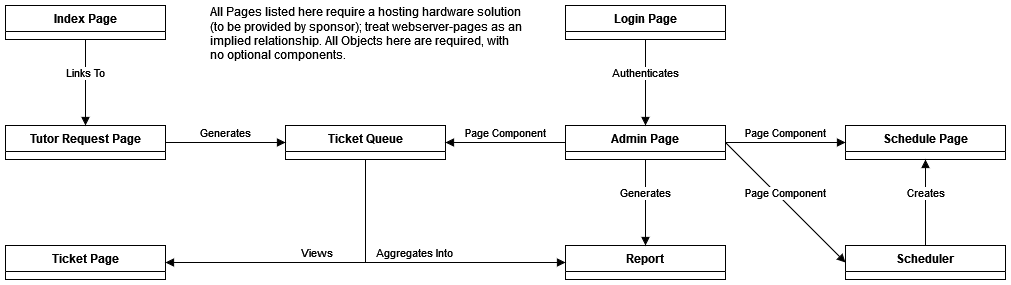
\includegraphics[width=160mm,scale=0.5]{img/UML Object Model.png}\\~\\

    \tab (add content)\\~\\
    {\color{red}Comment 3.3: Replace with deployment diagram, including Docker, NGINX. Describe the deployment process and tools (e.g., ngrok) you utilized.\\~\\}


    \section{Development View}
    \begin{itemize}
        \item discuss how the code is organized and how this organization is related to the previously identified subsystems
        \item discuss the role of the framework(s) used and how your code interacts with them
        \item identify which code modules or components were reused (e.g., open source libraries, existing code from another project, etc.)
        \item describe API calls to external services and third-party libraries
        \item corresponds to C4
        \item Links to an external site. Levels 3 and 4 diagrams
        \item 1 or more UML class diagrams are required
              \begin{itemize}
                  \item if there are 15 or less modules/classes, show interconnections between classes
                  \item if there are more than 15, use a UML package diagram to show the hierarchy
              \end{itemize}
    \end{itemize}

    \tab (add content)\\~\\
    {\color{red}Comment 3.4.1: Add separate diagrams for the frontend and backend showing the package structure down to React components and Python modules and the front and backend, respectively. \\~\\}
    {\color{red}Comment 3.4.2.	Explain how the classes are divided up and add rationale explaining why. For example, you can relate this to principles of modular design (e.g., separation of concerns, low coupling/high cohesion, etc) as well as requirements imposed by the frameworks used. Discuss also any alternative designs considered.\\~\\}


    \section{Data View}

    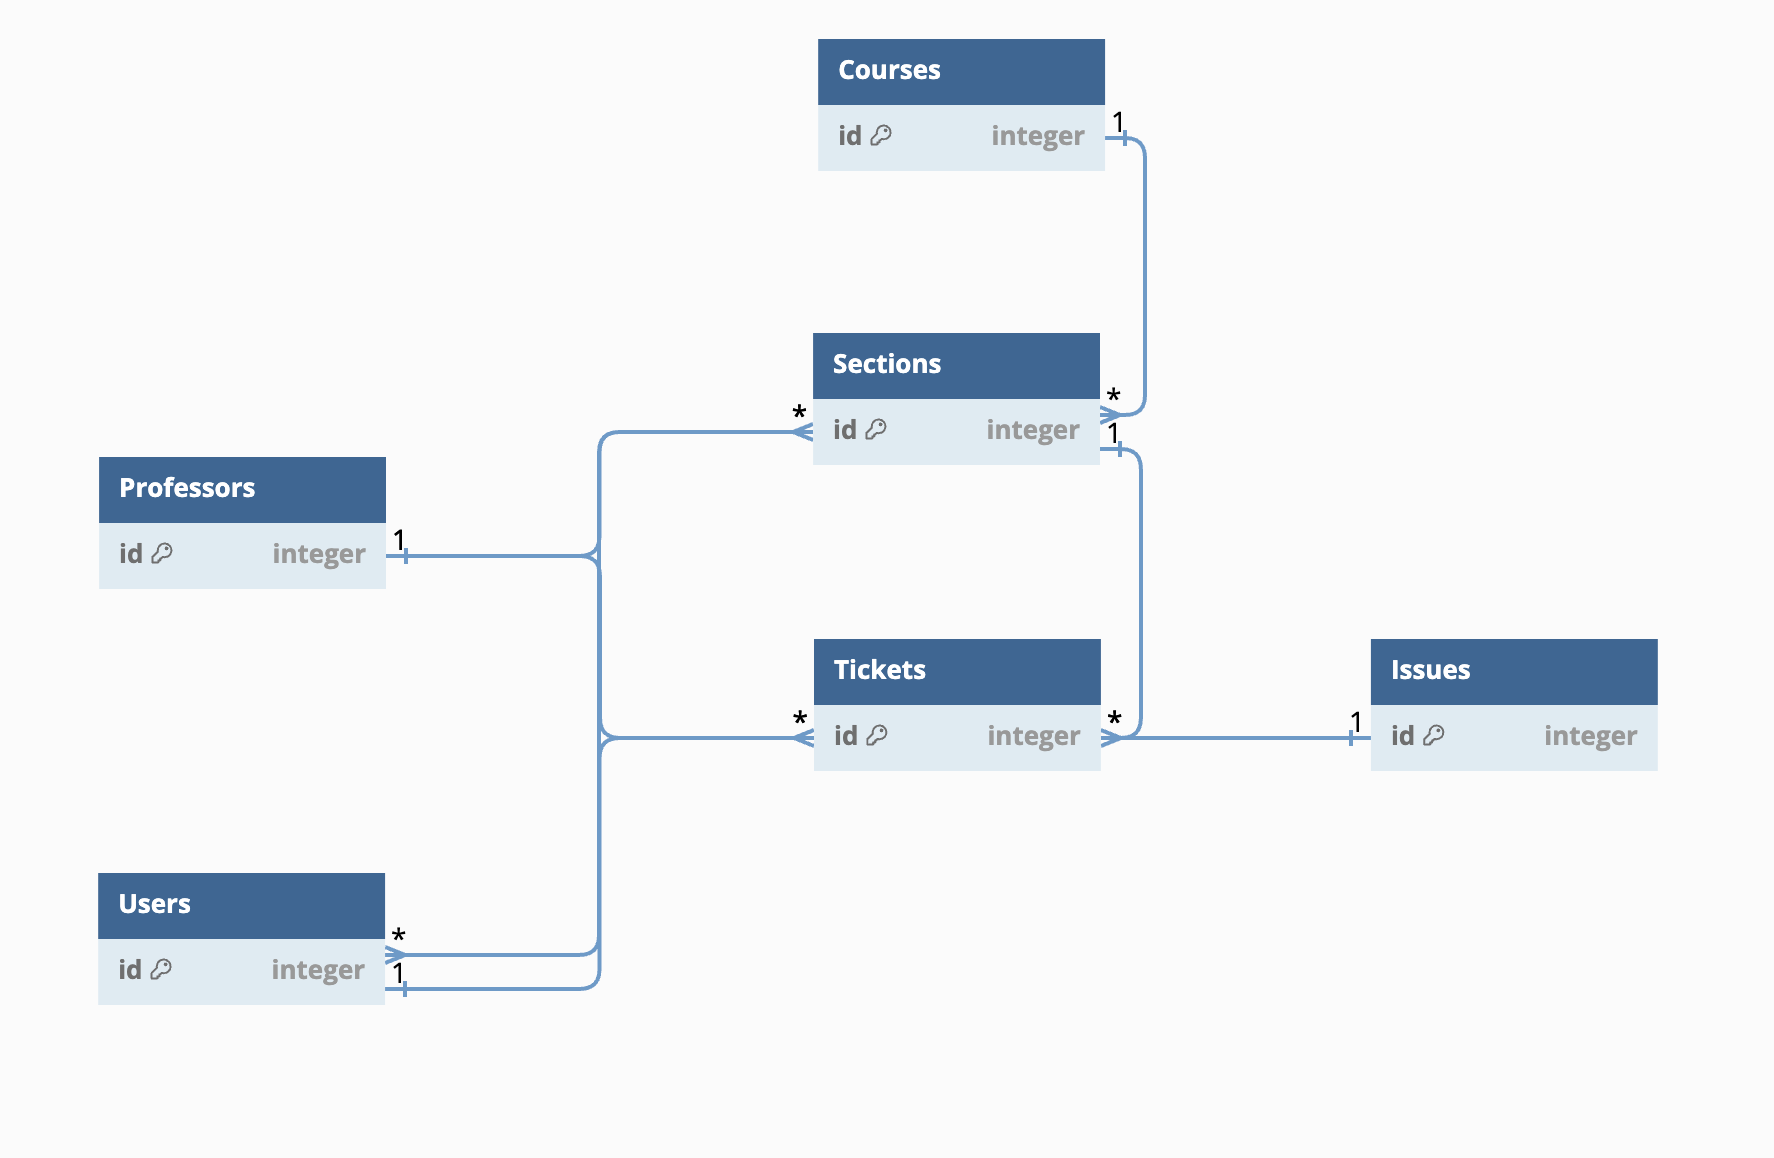
\includegraphics[width=160mm,scale=0.5]{img/relationship model.png}\\~\\

    %\begin{itemize}
    %    \item if relational db, describe the data tables and their relationships
    %    \item if not relational db, describe the object model
    %    \item if XML, JSON, etc. files, describe the schema
    %    \item other files that are saved should also be described here
    %    \item discuss the related code that uses each entity
    %\end{itemize}

    \tab Our current back-end relational database uses six tables. A More detailed version, and additional details will be made available in the final report.\\~\\
    {\color{red}Comment 3.5: Update to match final database implementation. \\~\\}

    \section{Concurrency View}

    \tab \TeamName\space does not anticipate work that would involve this section. we include this section as a placeholder and an acknowledgement that future work may re-scope us into this area.\\~\\


    \section{Execution Flow View}

    \begin{itemize}
        \item discuss illustrative scenarios that show data and control flow through the application modules to deliver a particular service
        \item 1 or more UML sequence diagrams are required
    \end{itemize}

    \tab (add content)\\~\\
    {\color{red}Comment 3.6.1:	For the execution flow view, show the interaction as sequence diagrams among the code modules from frontend to backend. Identify 1-2 scenarios from your functional requirements to illustrate the flow and use sequence diagrams to show how the execution flows from one module to another.  \\~\\}
    {\color{red}Comment 3.6.2: For one of the scenarios, illustrate how the web sockets push works.\\~\\}


    \section{Screenshots}

    \tab Below are several static captures of the website prior to deployment on UNO architecture. Some placeholder values and text are used.

    \begin{figure}
        \centering
        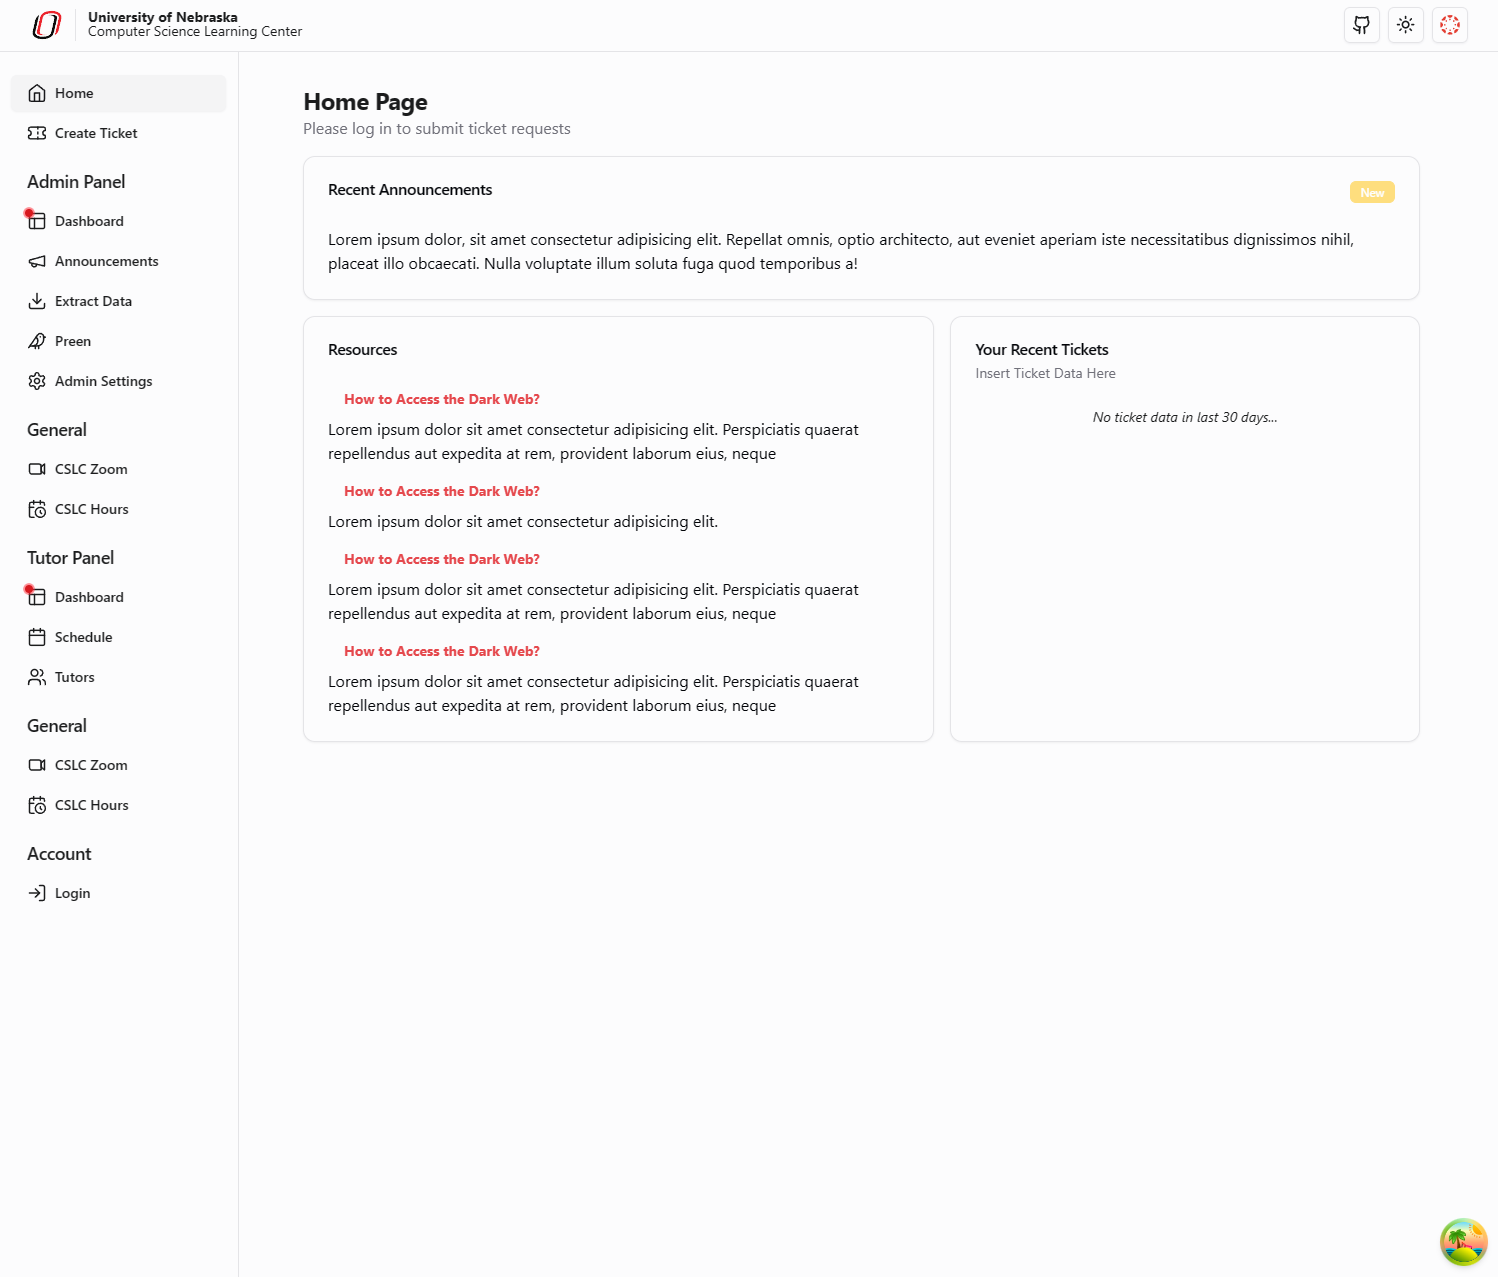
\includegraphics[width=0.75\linewidth]{img/Home Page.png}
        \caption{CSLC Home Page}
        \label{fig:Home Page}
    \end{figure}

    \begin{figure}
        \centering
        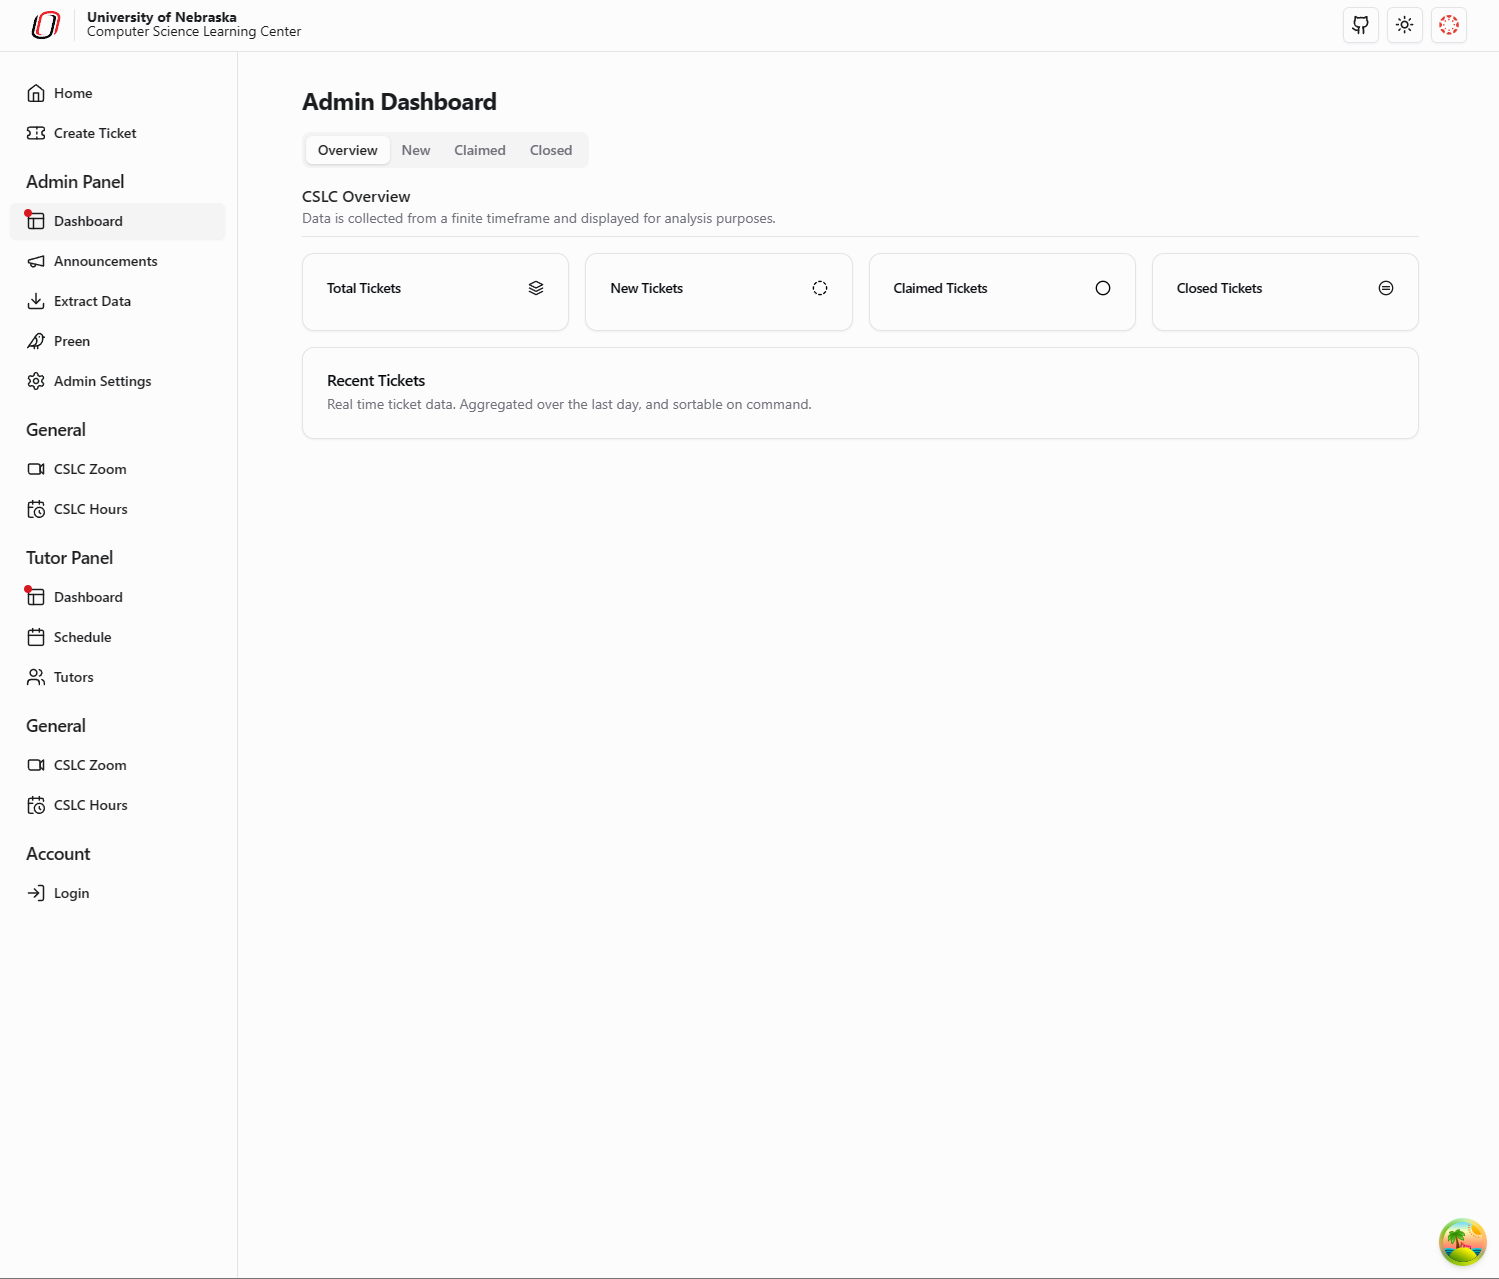
\includegraphics[width=0.75\linewidth]{img/Dashboard.png}
        \caption{CSLC Dashboard}
        \label{fig:Dashboard}
    \end{figure}

    \begin{figure}
        \centering
        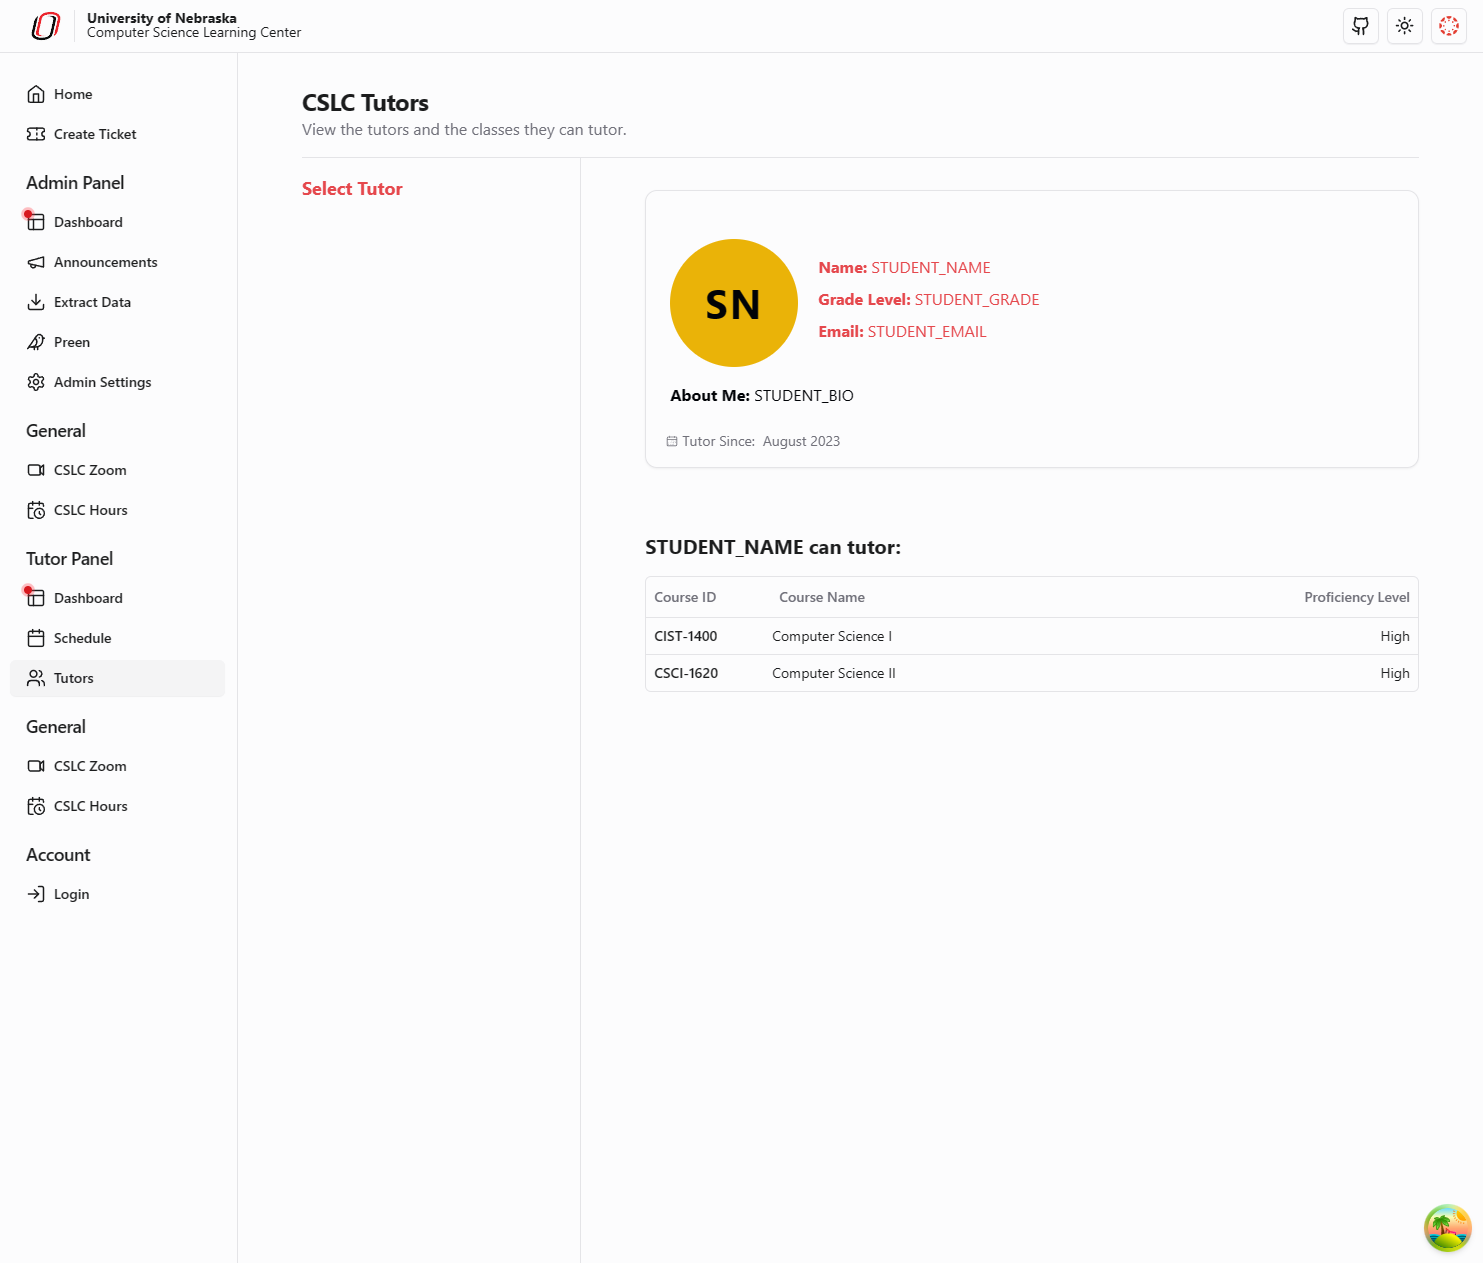
\includegraphics[width=0.75\linewidth]{img/Tutors.png}
        \caption{CSLC Tutor Page}
        \label{fig:Tutors Page}
    \end{figure}

    \begin{figure}
        \centering
        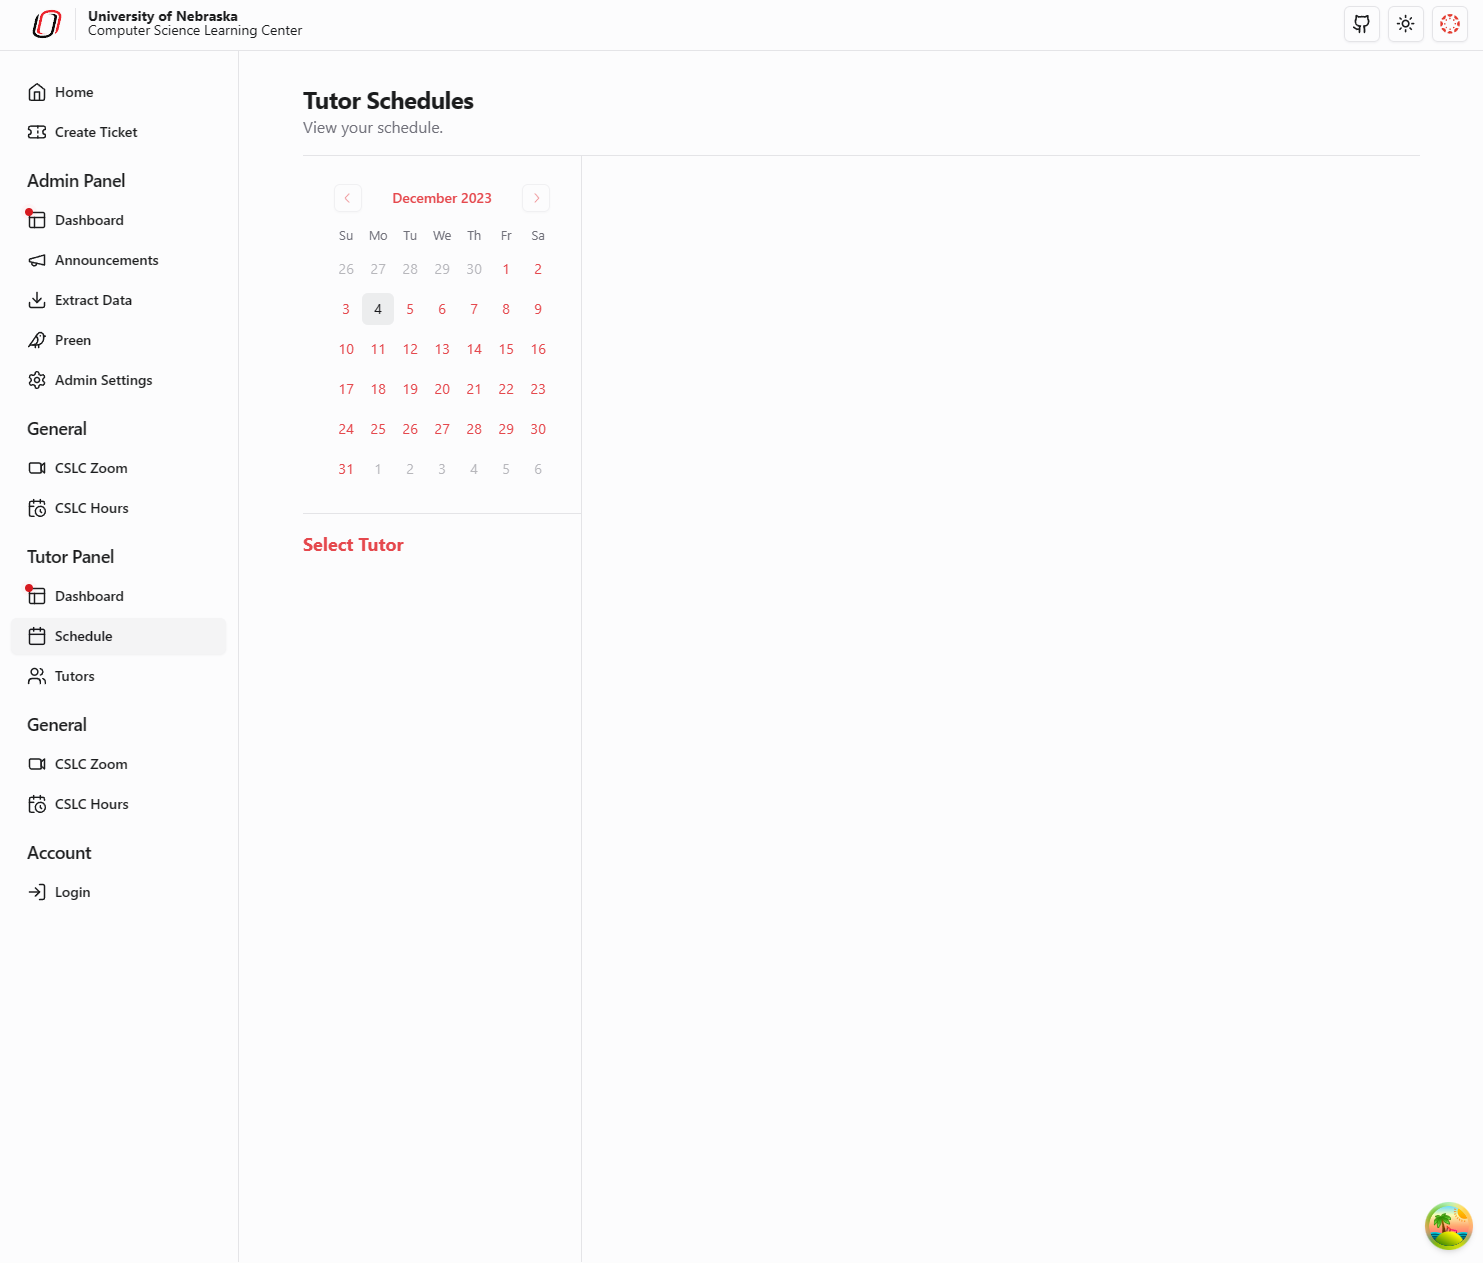
\includegraphics[width=0.75\linewidth]{img/Schedule.png}
        \caption{CSLC Schedule Page}
        \label{fig:Schedule Page}
    \end{figure}

    \begin{figure}
        \centering
        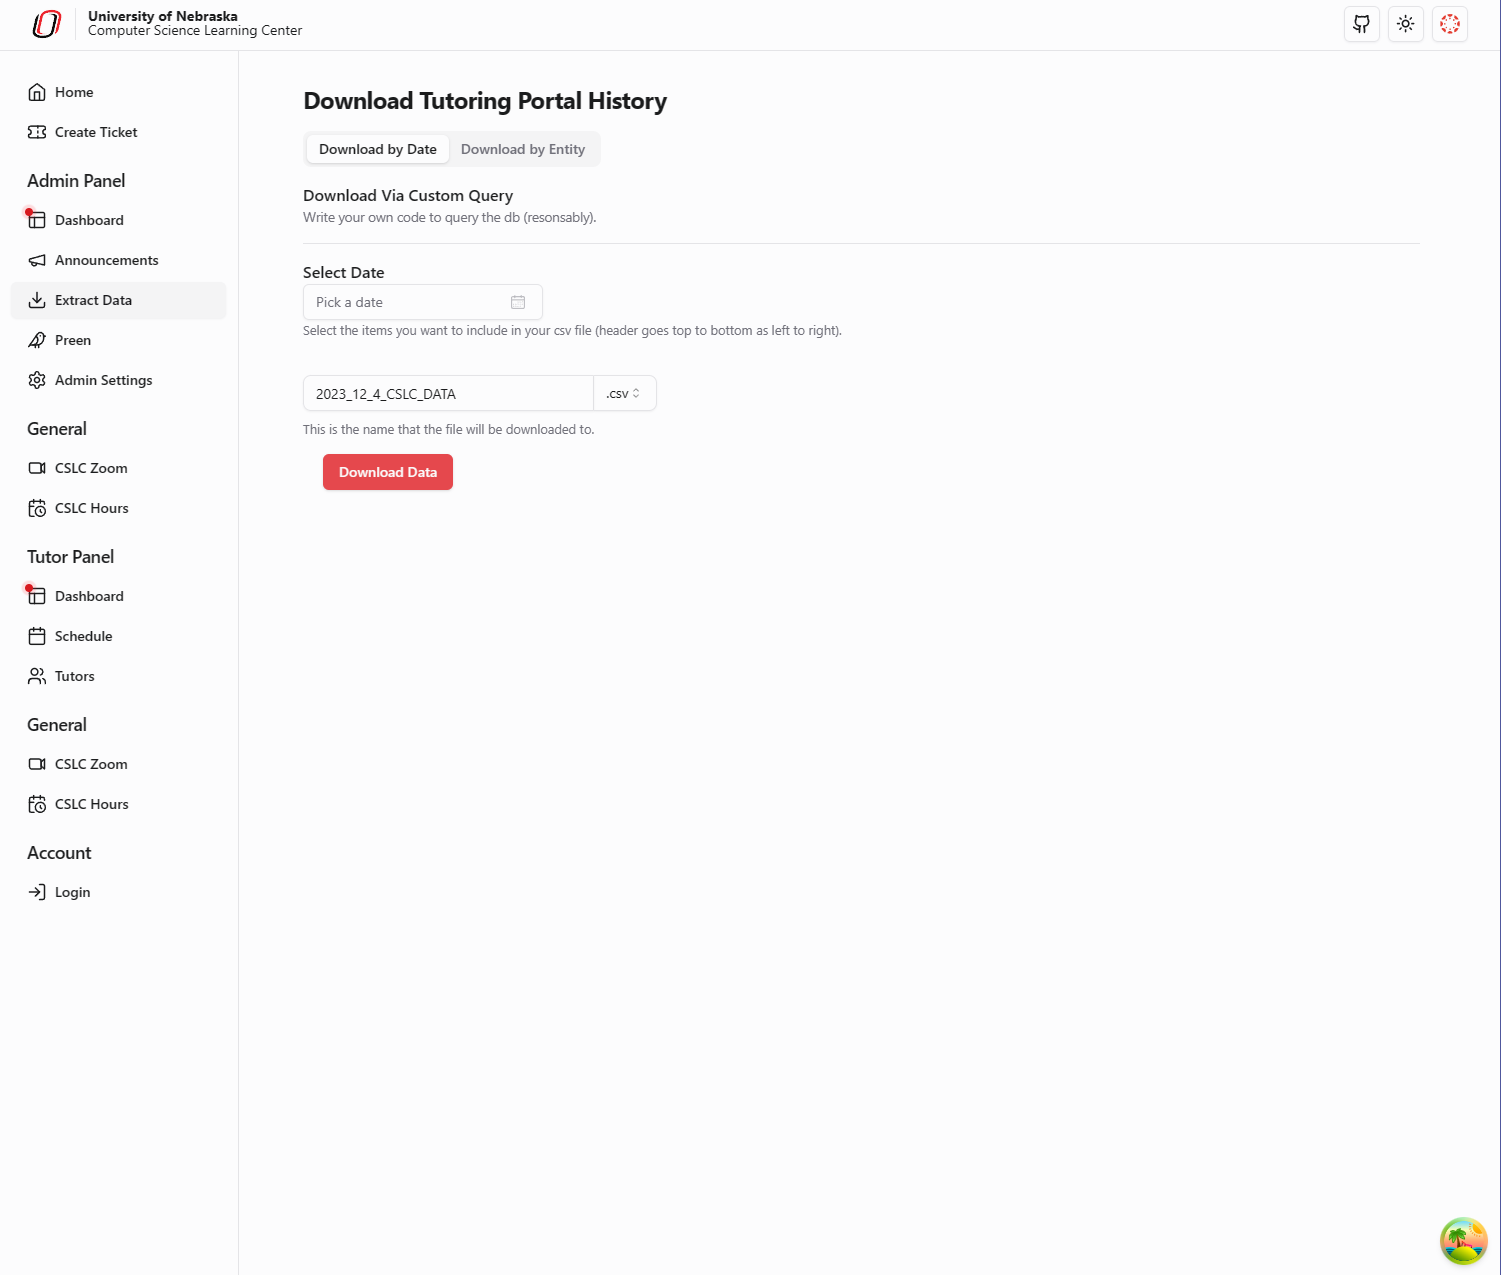
\includegraphics[width=0.75\linewidth]{img/Download.png}
        \caption{CSLC Download Page}
        \label{fig:Download Page}
    \end{figure}



    \section{Summary of Design Changes}

    \begin{itemize}
        \item summarize as applicable how the design has evolved from the original concept to the final version and explain the reason for the changes
    \end{itemize}

    \tab (TBD in Final Draft)\\~\\


    \section{Design Modularity and Extensibility}

    \tab A stretch goal \TeamName slated for work (but was unfortunately not accomplished within the scope of our work) was an integration with the registrar's office to automatically populate current IS\&T courses. Both the client and the \TeamName\space discussed this in our client meetings. While IS\&T has a table of courses, the upcoming changes in structure and shifting semester structure made this semester an inopportune time to tackle the issue.\\~\\

    \tab Future work would involve scoping and understanding the data's formatting requirements. A likely implementation would be an ingestion of a csv file through the admin portal. Via REST API, the csv data would populate a table in the back-end that would populate elements such as drop down menus for selecting a course on tutoring tickets.\\~\\
    {\color{red}Comment 3.7: In addition to describing the possible extensions, talk about your application's potential for extensibility. For example, what needs to change in your code to integrate with the registrar's class schedule system?\\~\\}
    {\color{blue}\tab acknowledging that this potential work is a likely future endeavor, we have attempted to structure our database around semesters markers. However as Kyle clarified, changes to back-end nomenclature on semesters may make database refactoring a necessity, despite our best effort. Any future implementations would likely involve re-keying the database or potentially archiving historic data and repopulating with a new schema and data.}


    \chapter{Implementation}

    \section{Directory Structure}

    \tab (TBD in Final Draft)\\~\\


    \section{Technical Issues Encountered}

    \tab (TBD in Final Draft)\\~\\
    {\color{red}Comment 4.1: Discuss any implementation task that took longer than expected, for example, web sockets. Discuss any issues that arose.  \\~\\}


    \section{User-Reported Bugs}

    \tab Due to scheduling conflicts with UNO's hosting subject matter experts, \TeamName has been unable to deploy the service on UNO's architecture. Consequently, wide-scale user testing has not been conducted. In lieu of this, we have done extensive unit testing.\\~\\




    \chapter{Testing}

    \section{Test Plan}
    \tab This test plan outlines the high level testing strategy for the CSLC Tutoring Portal. The primary objective of this testing plan is to ensure the robustness, functionality, and performance of the web application. This plan includes both integration testing and end-to-end testing, enabling our team to deliver a high performing web application that will meet the demands of the end users.\\~\\

    \tab In the integration testing scenario, we need to test the API integration and the component integration. With testing the API integration, we need to verify that the front-end properly communicates with the REST API back-end by testing API calls and responses for different endpoints. For component integration testing, Jest can be employed to ensure that the different web components of the application work together as expected. As Jest is primarily known for its unit testing, we plan to develop unit tests for our components to help identify potential bugs during the testing phase.\\~\\

    \tab The end-to-end testing approach in this plan is designed to comprehensively evaluate the users' journey from start to finish. We plan on using Selenium to stimulate users actions such as clicks and inputs to asses the application's performance. Additionally, Selenium can be used for cross-browser compatibility testing to ensure that our application works across a variety of browsers. Similar to the integration testing, the end-to-end testing process is focused on identifying any potential bugs during the testing phase, ensuring the delivery of a dependable and user-friendly application.\\~\\
    {\color{red}Comment 5.1: Looks good. Update as needed to reflect how testing was carried out.\\~\\}


    \section{Obtaining Realistic Test Data}

    \tab (TBD in Final Draft)\\~\\


    \section{Tests Conducted}

    \tab (TBD in Final Draft)\\~\\


    \section{Test Results}

    \tab (TBD in Final Draft)\\~\\


    \section{Automated Test Outputs}

    \tab (TBD in Final Draft)\\~\\


    \section{Tests Not Conducted}

    \tab (TBD in Final Draft)\\~\\





    \chapter{Summary}

    \section{Summary of Project Organization}

    \tab \TeamName largely upheld the initially outlined roles, as our record-keeping reflects.Throughout the course of Work, Nolan maintained his roles as  the architect, technical lead, back-end developer and dev-ops and database developer. Nolan was continually the lead developer, working with Lindsey as the UI/UX and front-end \& mobile lead to develop the code base. Mya and Austin worked as client liaison and quality assurance testers. Mya oversaw large portion of the requirements chapter as the requirements analyst.\\~\\

    \section{Outcome of Risks}

    \tab (TBD in Final Draft)\\~\\


    \section{Milestone Summary}

    \tab (TBD in Final Draft)\\~\\


    \section{Lessons Learned}

    \tab (TBD in Final Draft)\\~\\


    \section{Future Extensions}

    \tab (TBD in Final Draft)\\~\\




    \chapter{Local and Global Impacts}

    \tab The establishment of the IS\&T's CSLC is a transformative initiative with far-reaching positive impacts, both locally and globally. This tutoring center, designed to harness the intellectual prowess of students within the university, not only contributes to the academic success of individuals but also serves as a catalyst for societal advancement.\\~\\

    \tab At its core, the CSLC plays a pivotal role in building academic excellence within IS\&T. By providing a dedicated space for students to receive personalized tutoring in various technology courses, the center becomes a nexus of knowledge and collaboration. The employment of student tutors ensures a relatable and accessible learning environment, fostering a sense of camaraderie and peer support. This not only enhances the academic performance of the tutored students but also cultivates a culture of knowledge-sharing and mentorship within the university.\\~\\

    \tab One of the immediate local impacts is the empowerment of students to overcome academic challenges. As the CSLC aids in comprehension and mastery of complex computing concepts, it acts as a springboard for students to excel in their coursework. This success, in turn, contributes to the overall reputation of the college, attracting prospective students and faculty, thereby bolstering the academic community.\\~\\

    \tab On a global scale, the CSLC contributes to the advancement of information science and technology. In an era where computing applications have become ubiquitous and integral to various aspects of society, the center becomes a hub for cultivating the next generation of tech leaders. Graduates of the College of IS\&T, shaped by the support and guidance received at the CSLC, are poised to make meaningful contributions to client organizations, local communities, and business and industrial communities worldwide.\\~\\

    \tab The positive impact of the CSLC extends beyond academic success. It serves as a cornerstone for the development of well-rounded individuals who not only excel in their chosen field but also understand the broader implications of their work on society. As computing applications continue to shape the fabric of our interconnected world, the CSLC emerges as a beacon of education, collaboration, and societal progress within the realm of information science and technology.\\~\\





    % .----------------.  .----------------.  .----------------.  .----------------.  .-----------------. .----------------.  .----------------.  .----------------. 
    %| .--------------. || .--------------. || .--------------. || .--------------. || .--------------. || .--------------. || .--------------. || .--------------. |
    %| |      __      | || |   ______     | || |   ______     | || |  _________   | || | ____  _____  | || |  ________    | || |     _____    | || |  ____  ____  | |
    %| |     /  \     | || |  |_   __ \   | || |  |_   __ \   | || | |_   ___  |  | || ||_   \|_   _| | || | |_   ___ `.  | || |    |_   _|   | || | |_  _||_  _| | |
    %| |    / /\ \    | || |    | |__) |  | || |    | |__) |  | || |   | |_  \_|  | || |  |   \ | |   | || |   | |   `. \ | || |      | |     | || |   \ \  / /   | |
    %| |   / ____ \   | || |    |  ___/   | || |    |  ___/   | || |   |  _|  _   | || |  | |\ \| |   | || |   | |    | | | || |      | |     | || |    > `' <    | |
    %| | _/ /    \ \_ | || |   _| |_      | || |   _| |_      | || |  _| |___/ |  | || | _| |_\   |_  | || |  _| |___.' / | || |     _| |_    | || |  _/ /'`\ \_  | |
    %| ||____|  |____|| || |  |_____|     | || |  |_____|     | || | |_________|  | || ||_____|\____| | || | |________.'  | || |    |_____|   | || | |____||____| | |
    %| |              | || |              | || |              | || |              | || |              | || |              | || |              | || |              | |
    %| '--------------' || '--------------' || '--------------' || '--------------' || '--------------' || '--------------' || '--------------' || '--------------' |
    % '----------------'  '----------------'  '----------------'  '----------------'  '----------------'  '----------------'  '----------------'  '----------------'           

    \chapter{Appendix}

    \vspace{1.5cm}
    \begin{center}
        \textit{This Page is intentionally left blank}
    \end{center}
    \newpage
    %\section{Project Proposal}

    \stepcounter{section}\addcontentsline{toc}{section}{\protect\numberline{\thesection}{Project Proposal}}

    
\includepdf[pages=-, scale=0.80, frame=true, pagecommand={\begin{center}Project Proposal\end{center}}]{pdf/Project Proposal.pdf}


    \stepcounter{section}\addcontentsline{toc}{section}{\protect\numberline{\thesection}{Project Plan}}

    
\includepdf[pages=-, scale=0.80, frame=true, pagecommand={\begin{center}Project Plan\end{center}}]{pdf/Project Plan.pdf}


    \stepcounter{section}\addcontentsline{toc}{section}{\protect\numberline{\thesection}{Initial Requirements}}

    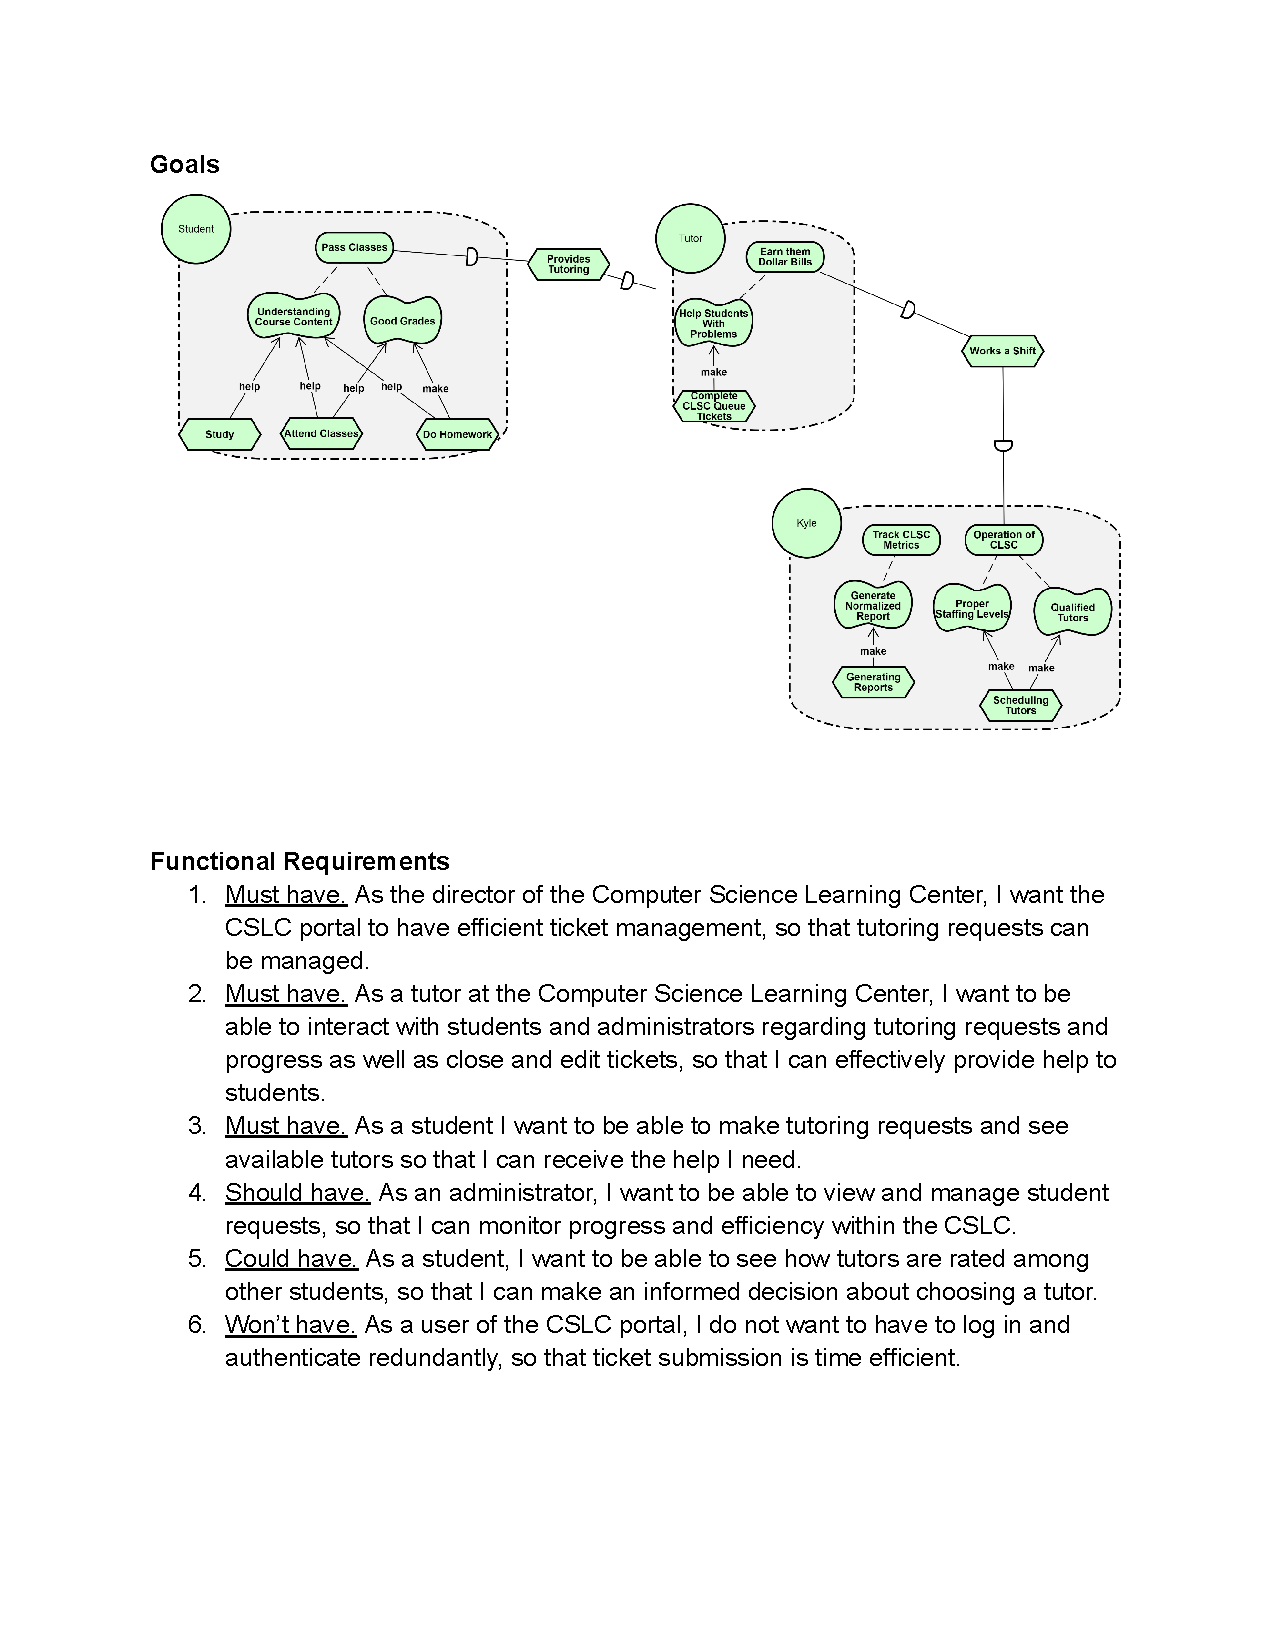
\includepdf[pages=-, scale=0.80, frame=true, pagecommand={\begin{center}Initial Requirements\end{center}}]{pdf/Initial Requirements.pdf}


    \stepcounter{section}\addcontentsline{toc}{section}{\protect\numberline{\thesection}{Context Document}}

    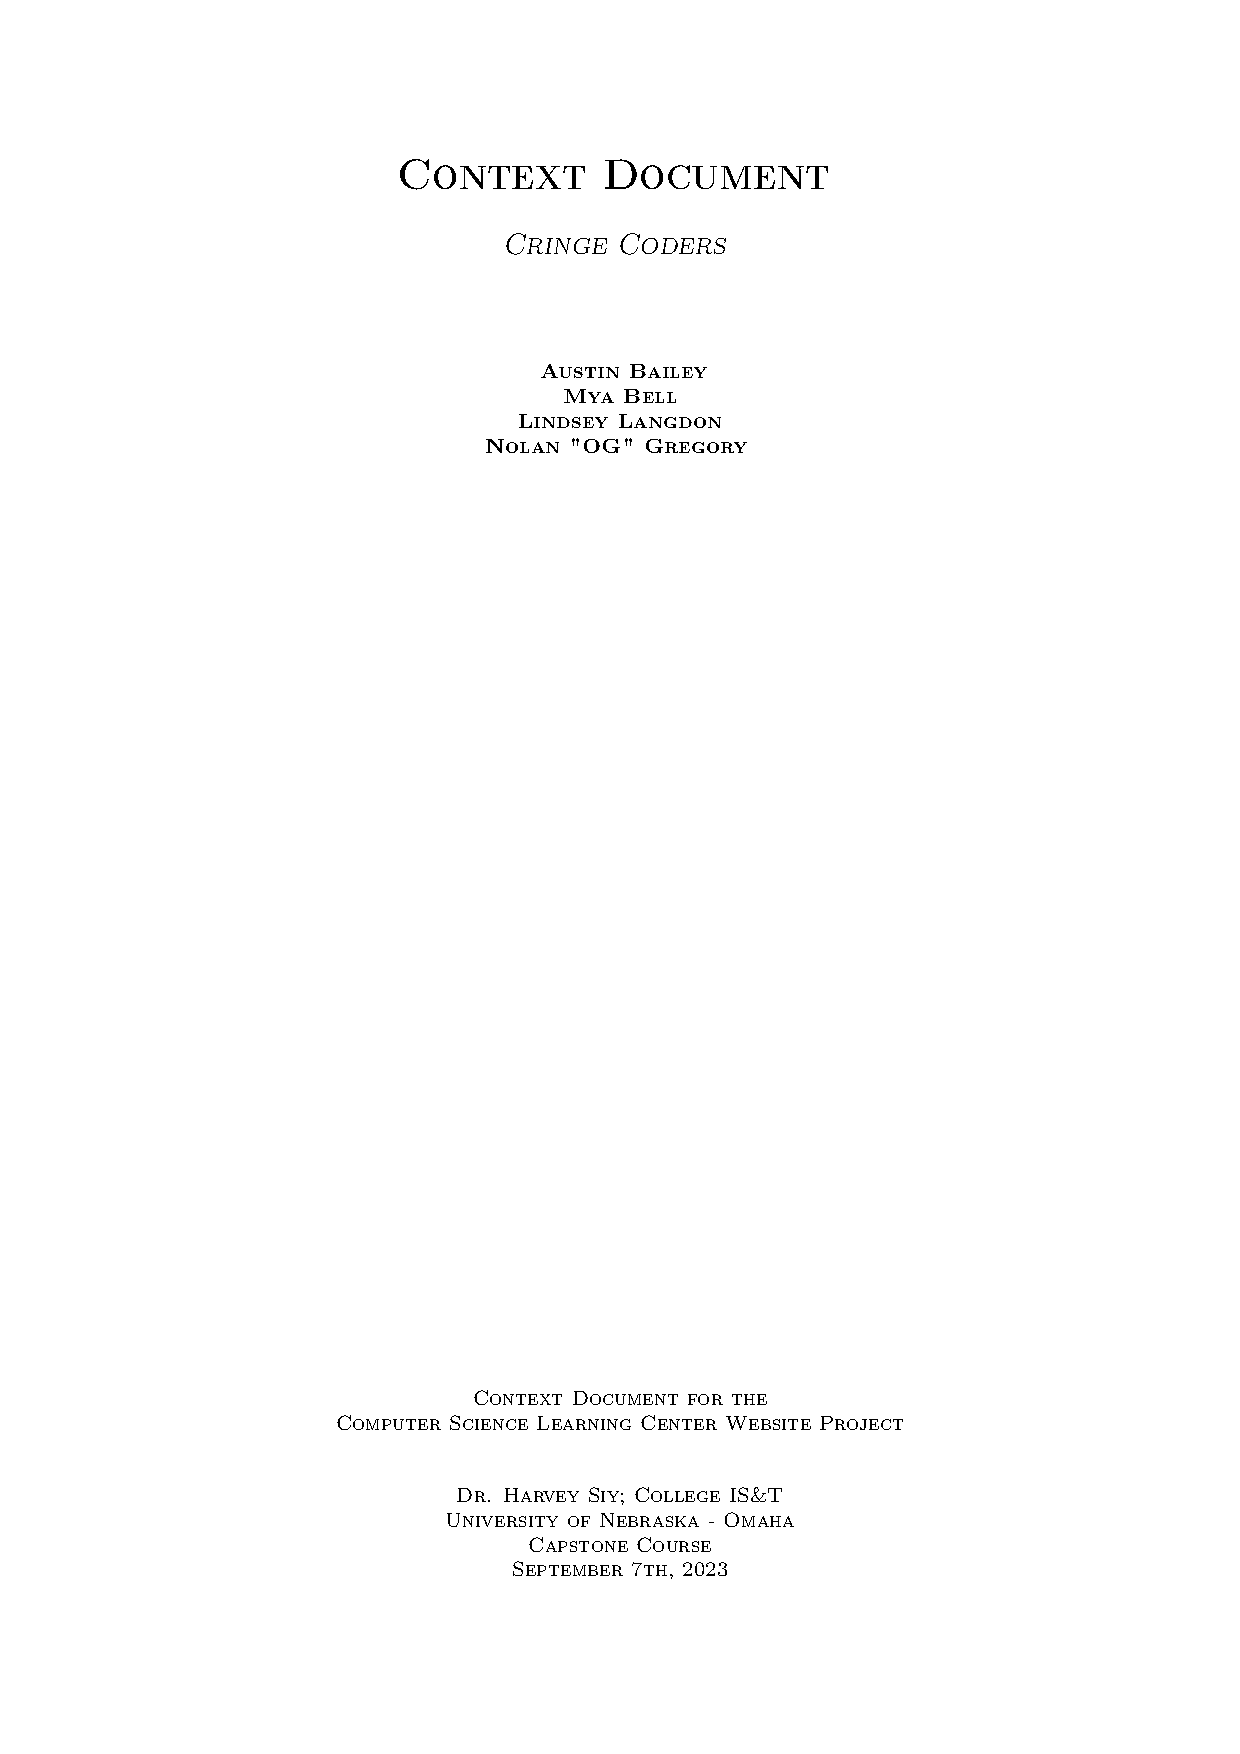
\includepdf[pages=-, scale=0.80, frame=true, pagecommand={\begin{center}Context Document\end{center}}]{pdf/Context Document.pdf}


    \stepcounter{section}\addcontentsline{toc}{section}{\protect\numberline{\thesection}{Mid Semester Project Report}}

    \includepdf[pages=1-18, scale=0.80, frame=true, pagecommand={\begin{center}Mid Semester Project Report\end{center}}]{pdf/Mid Semester Report.pdf}


    \section{Setup \& Deployment Instructions}

    \tab The most detailed and up to date instructions for deploying the project are available through the GitHub repository:\space\url{https://github.com/nulzo/University-Nebraska-Tutor-Portal}. The as-is rendering the markdown instructions is given below for the sake of completeness.

    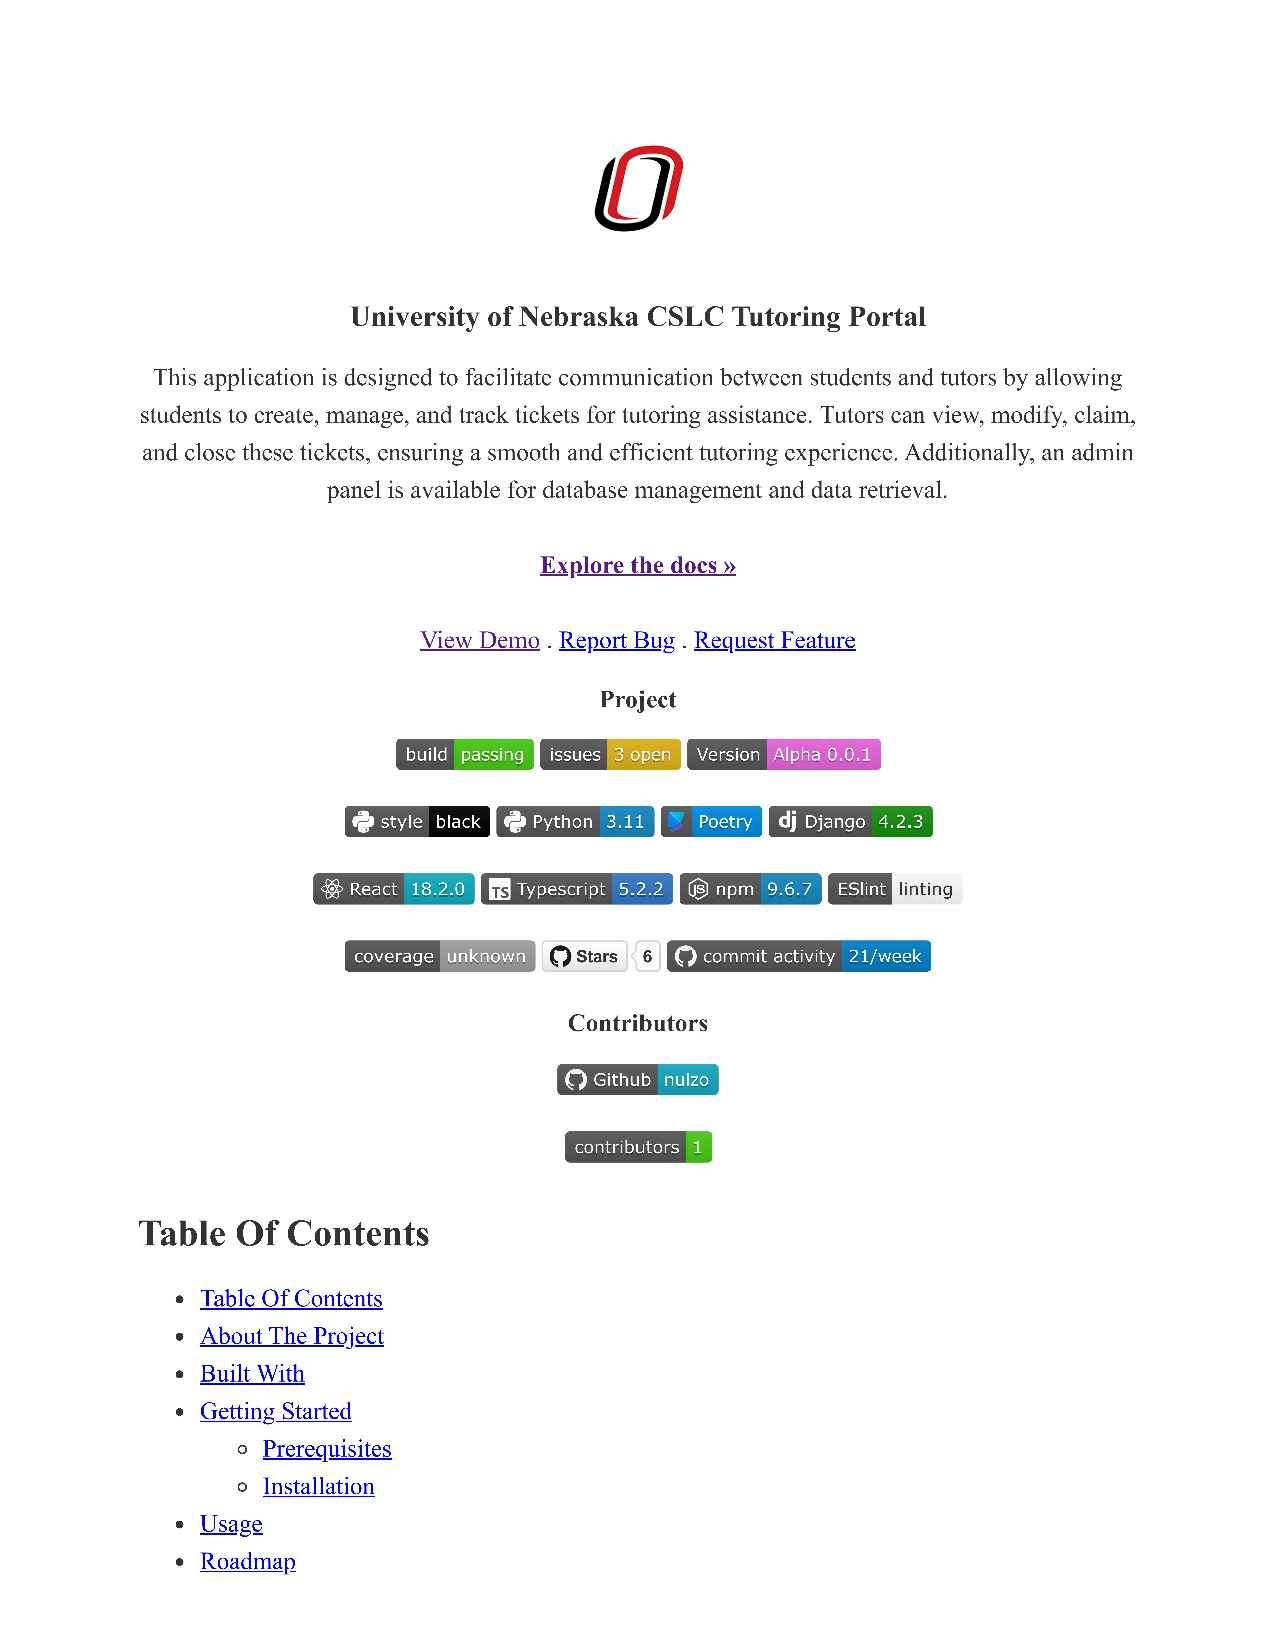
\includepdf[pages=-, scale=0.80, frame=true, pagecommand={\begin{center}Github README.md Instructions \textit{(As of 26-Nov-23)}\end{center}}]{pdf/README.pdf}


    \section{Team Meeting Notes}

    \tab Sans the initial client meeting, the \TeamName\space has felt no sense of urgency or disconnect between us and our client that would necessitate extra-ordinary meetings outside of class time. Consequently, we have held no meetings outside of class times, and our meetings during class time typically span about five minutes. Therefore, we have neglected to keep a record of internal team meeting notes.\\~\\
    \tab We do have a record and transcription of our initial client meeting attached in the appendix separate from our team meetings, and we do have the below interaction with out client Kyle. Much, if not all of the intended content, such as assignment of work and completion of work are readily implied by the \TeamName's individual journals.\\~\\
    \begin{center}
        \def\arraystretch{2.5}
        \begin{longtable}{ p{1.5cm} p{13.5cm} }
            \multicolumn{2}{c}{\large\textit{October 3rd Mid-Semester Meeting Scheduling}}                                                                                                                                                                                                                                                                                                                                                                                                                                                                                                                                                                                                                                    \\ \hline
            \textbf{\textit{Nolan}} & Hey [Kyle]! Hope everything has been going well these past few weeks. We have made some pretty solid progress on the portal so far. During our first meeting we talked about meeting up sometime around mid-October for another, so I was just reaching out to get a date figured out. I think fall break is in two weeks, so would you have availability to meet up sometime next week? I think the best time for our group is Tuesday/Thursday from 1:00-1:30 or sometime around 2:00ish - it's hard to tell how long Harvey will lecture for. Just let us know if any of those times work for you, and we can figure something else out if you're booked during those times. thanks! \\

            \textbf{\textit{Kyle}}  & Well, I don't know if any of you are going out of town for Fall Break, but I could do the Tuesday during it (the 17th) in the afternoon and then you wouldn't have to worry about when the lecture gets out. If not, we could do that Thursday (the 19th).                                                                                                                                                                                                                                                                                                                                                                                                                              \\
                                    & Also I forgot to give the order I was wanting the reports to be in. Here is that order: URL, Student Email, Student First Name, Student Last Name, Assignment, Question, Problem Type, Status, Time Created, Time Closed, Was Successful, Primary Tutor, Assistant Tutor, Semester, Course Number, Section Number, Professor, ANYTHING NEW                                                                                                                                                                                                                                                                                                                                              \\
                                    & And the url it should use: \url{https://cslc.unomaha.edu/}                                                                                                                                                                                                                                                                                                                                                                                                                                                                                                                                                                                                                              \\

            \textbf{\textit{Nolan}} & Hey Kyle, I have spoken with the group and I believe Thursday will work best as some team members have plans for the midterm break. I'd be happy to meet you in your office or at the CSLC or something and pick out a time that works!                                                                                                                                                                                                                                                                                                                                                                                                                                                 \\

                                    & Also, we have some exciting news to share: Harvey looks to have gotten some VMs for us to use, so hopefully we can get that figured out so you can have an easy test environment to mess around with instead of pulling down and running docker containers :) I'll keep you posted with that, still need to figure out exactly how he has them set up!                                                                                                                                                                                                                                                                                                                                  \\

                                    & Looking forward to seeing you soon, and let us know if you have any questions in the meantime :) have a good weekend!                                                                                                                                                                                                                                                                                                                                                                                                                                                                                                                                                                   \\ \hline
        \end{longtable}
    \end{center}


    \section{Individual Journals}

    \subsection{Austin Bailey}

    \textit{Client Liaison\\
        Information Security Analyst\\
        Quality Assurance Tester\\~\\}

    \tab Austin Bailey is responsible for thoroughly testing the application to identify vulnerabilities, usability issues, and performance bottlenecks. Austin will create and execute test cases, provide feedback to the development team, and ensure a high-quality final product. Likewise, Austin will simulate real-world cyberattacks to identify vulnerabilities and weaknesses. Austin will help our team improve our security posture and protect sensitive information by uncovering any potential security flaws.\\~\\

    \textbf{Journal\\}
    8/31 - built project context with lindsey\\
    9/05 - met with client; record and will transcribe\\
    9/07 - met helped build context document\\
    9/12 - record context document with Mya\\
    9/14 - Attended class; Built a goal model; provided pen + paper for wire framing\\
    9/19 - Attended class; consolidated documents for submitting to canvas with team; scoped work\\
    \tab of UML diagram to be done by EOD thursday (9/21)\\
    9/21 - attended class\\
    9/26 - Weekly Meeting with Siy; attended class\\
    9/28 - Attended class\\
    10/03 - Coordinated with Nolan for follow-up meeting with client; attended class\\
    10/05 - no changes to project; team agreed no changes were necessary. Attended class\\
    10/10 - context document formalization; project report work; attended class\\
    10/12 - Mid-semester Project report finalization\\
    10/17 - Fall Break
    10/19 - Client meeting; recorded meeting; attended class\\
    10/24 - Attended Class; Studying for MFT; Formatting transcript\\
    10/26 - Attended Class; Professor Check-In; Studying for MFT; Formatting transcript\\
    10/31 - Attended Class; Formatting transcript\\
    11/02 - Attended Class; Professor Check-In; Addressed any IP concerns (N/A)\\
    11/07 - Attended Class; Formatting transcript\\
    11/09 - Attended Class; Professor Check-In\\
    11/14 - Attended Class\\
    11/16 - Attended Class; Professor Check-In\\
    11/21 - Finalizing transcript \\
    11/23 - Thanksgiving \\
    11/28 - Attended Class; Review mid-semester report comments; Begin drafting final report \\
    11/30 - Attended Class; Professor Check-In; drafting final report \\~\\

    \subsection{Mya Bell}

    \textit{Client Liaison\\
        Requirements Analyst\\
        Quality Assurance Tester\\~\\}

    \tab Mya Bell will oversee the development process, and ensure that the project stays on track, objectives are met, and communication flows smoothly between team members. Likewise, Mya will facilitate communication and collaboration between leadership and team players to ensure a successful outcome. Lastly, Mya will create and execute test cases to ensure a high-quality final product.\\~\\

    \textbf{Journal\\}
    August 31 - Discussed and finalized individual roles, project proposal, and project plan\\
    September 5 - First meeting with client\\
    September 7 - Wrote and recorded context document\\
    September 12 - Wrote initial requirements document\\
    September 14 - Finished requirements document\\
    September 19 - Started nonfunctional requirements\\
    September 21 - Discussed object model and finished nonfunctional requirements and updated requirements\\
    September 26 - Went over progress on code milestone 1\\
    September 28 - Check in with Mr. Siy\\
    October 3 - Updated client on progress and scheduled next meeting with client\\
    October 5 - Check in with Mr. Siy and reviewed current project plan\\
    October 10 - Automated testing tools demo\\
    October 12 - Check in with Mr. Siy and worked on midsemester project report\\~\\

    \subsection{Nolan Gregory}
    \textit{Architect\\
        Technical Lead\\
        Back-End Developer\\
        Dev-Ops and Database\\~\\}

    \tab Nolan Gregory is responsible for making technical decisions and guiding the development process. Nolan will provide technical expertise, review code, and ensure that the architecture and technologies chosen align with the project's goals. Nolan will handle all server-side logic, database management, and API calls. Nolan will build the core functionalities of the application, including ticket management, user authentication, and communication features. Nolan will design and maintain the database structure, ensuring efficient data storage, retrieval, and integrity. Lastly, Nolan will set up the deployment infrastructure, manage continuous integration/continuous deployment (CI/CD) pipelines, and ensures smooth deployment and scaling of the ticketing portal.\\~\\

    \textbf{Journal\\}
    (add content)\\~\\

    \subsection{Lindsey Langdon}

    \textit{UI/UX Lead\\
        Front-End Developer\\
        Mobile Design Lead\\~\\}

    \tab Lindsey Langdon is responsible for creating an intuitive and visually appealing user interface. Lindsey will design wireframes, mockups, and prototypes, ensuring a user-friendly experience and consistent branding. Lindsey will be responsible for implementing the user interface and ensuring that the application is responsive and visually engaging. They work closely with the UI/UX Designer to translate design concepts into functional front-end components. Lindsey will ensure that the front-end can run on mobile or tablet devices, as well as on desktop systems, with a focus on mobile-first design.\\~\\

    \textbf{Journal\\}
    8/31 - built project context with Austin and worked on Project Proposal\\
    9/5 - went over client meeting notes\\
    9/7 - worked on wireframing exercises\\
    9/12 - assisted with writing context documentation\\
    9/14 - recorded Wireframes and Goal Model Requirements presentations\\
    9/19 - worked on GQM Modeling\\
    9/21 - attended class\\
    9/26 - weekly Meeting with Siy\\
    9/28 - attended class\\
    10/3 - attended class\\
    10/5 - team agreement that there were no changes to project plan\\
    10/10 -  recorded Testing Tool Demo presentation\\
    10/12 - worked on Mid-semester Project report\\~\\


    \section{Transcripts of Client Meetings}

    \stepcounter{subsection}\addcontentsline{toc}{subsection}{\protect\numberline{\thesubsection}{Transcript of Initial Client Meeting}}

    
\includepdf[pages=-, scale=0.80, frame=true, pagecommand={\begin{center}Transcript of Initial Client Meeting\end{center}}]{pdf/Transcript.pdf}

    \stepcounter{subsection}\addcontentsline{toc}{subsection}{\protect\numberline{\thesubsection}{Transcript of 19 October Client Check-In Meeting}}

    
\includepdf[pages=-, scale=0.80, frame=true, pagecommand={\begin{center}Transcript of 19 October Client Check-In\end{center}}]{pdf/Transcript of 19 October Client Check-In.pdf}

    \stepcounter{subsection}\addcontentsline{toc}{subsection}{\protect\numberline{\thesubsection}{Transcript of the Turbo Encabulator Meeting}}

    
\includepdf[pages=-, scale=0.80, frame=true, pagecommand={\begin{center}Transcript of the Turbo Encabulator Meeting\end{center}}]{pdf/Turbo Encabulator.pdf}

    \section{Rasterized Documentation of Module Interfaces}

    \tab The documentation for the CSLC portal was created via Sphinx. Here, we use the python package \texttt{weasyprint} to crudely cast the html documentation into a pdf format for the sake of appending a static copy to the final report. This is not meant as a replacement to Sphinx's html documentation; instead, the pdf renderings provide proof of work. We converted the html files to pdf by running the following bash commands:\\~\\
    \begin{lstlisting}    
find -name "*.html" | while read -r file; do 
    weasyprint "\$file" "./\${file}.pdf"; 
done\end{lstlisting}

    \tab This documentation is provided as-is of the 26th November, 2023. For the most up to date version, please see the github and generate the Sphinx documentation via the \texttt{make html} in the \url{/docs} directory. Not only will that version be more up to date, but the UI will look better, as Sphinx documentation is designed to be viewed in a web browser, not as a pdf.

    \newcommand\paper{Sphinx/about.html.pdf}
    \stepcounter{subsection}\addcontentsline{toc}{subsection}{\protect\numberline{\thesubsection}{\paper}}

    \includepdf[pages=2-, scale=0.80, frame=true, pagecommand={\begin{center}\paper\end{center}}]{\paper}

    \renewcommand\paper{Sphinx/course.html.pdf}
    \stepcounter{subsection}\addcontentsline{toc}{subsection}{\protect\numberline{\thesubsection}{\paper}}

    \includepdf[pages=2-, scale=0.80, frame=true, pagecommand={\begin{center}\paper\end{center}}]{\paper}

    \renewcommand\paper{Sphinx/genindex.html.pdf}
    \stepcounter{subsection}\addcontentsline{toc}{subsection}{\protect\numberline{\thesubsection}{\paper}}

    \includepdf[pages=2-, scale=0.80, frame=true, pagecommand={\begin{center}\paper\end{center}}]{\paper}

    \renewcommand\paper{Sphinx/index.html.pdf}
    \stepcounter{subsection}\addcontentsline{toc}{subsection}{\protect\numberline{\thesubsection}{\paper}}

    \includepdf[pages=2-, scale=0.80, frame=true, pagecommand={\begin{center}\paper\end{center}}]{\paper}

    \renewcommand\paper{Sphinx/index.html.pdf}
    \stepcounter{subsection}\addcontentsline{toc}{subsection}{\protect\numberline{\thesubsection}{\paper}}

    \includepdf[pages=2-, scale=0.80, frame=true, pagecommand={\begin{center}\paper\end{center}}]{\paper}

    \renewcommand\paper{Sphinx/issue.html.pdf}
    \stepcounter{subsection}\addcontentsline{toc}{subsection}{\protect\numberline{\thesubsection}{\paper}}

    \includepdf[pages=2-, scale=0.80, frame=true, pagecommand={\begin{center}\paper\end{center}}]{\paper}

    \renewcommand\paper{Sphinx/load-semester.html.pdf}
    \stepcounter{subsection}\addcontentsline{toc}{subsection}{\protect\numberline{\thesubsection}{\paper}}

    \includepdf[pages=2-, scale=0.80, frame=true, pagecommand={\begin{center}\paper\end{center}}]{\paper}

    \renewcommand\paper{Sphinx/modules.html.pdf}
    \stepcounter{subsection}\addcontentsline{toc}{subsection}{\protect\numberline{\thesubsection}{\paper}}

    \includepdf[pages=2-, scale=0.80, frame=true, pagecommand={\begin{center}\paper\end{center}}]{\paper}

    \renewcommand\paper{Sphinx/professor.html.pdf}
    \stepcounter{subsection}\addcontentsline{toc}{subsection}{\protect\numberline{\thesubsection}{\paper}}

    \includepdf[pages=2-, scale=0.80, frame=true, pagecommand={\begin{center}\paper\end{center}}]{\paper}

    \renewcommand\paper{Sphinx/py-modindex.html.pdf}
    \stepcounter{subsection}\addcontentsline{toc}{subsection}{\protect\numberline{\thesubsection}{\paper}}

    \includepdf[pages=2-, scale=0.80, frame=true, pagecommand={\begin{center}\paper\end{center}}]{\paper}

    \renewcommand\paper{Sphinx/search.html.pdf}
    \stepcounter{subsection}\addcontentsline{toc}{subsection}{\protect\numberline{\thesubsection}{\paper}}

    \includepdf[pages=2-, scale=0.80, frame=true, pagecommand={\begin{center}\paper\end{center}}]{\paper}

    \renewcommand\paper{Sphinx/section.html.pdf}
    \stepcounter{subsection}\addcontentsline{toc}{subsection}{\protect\numberline{\thesubsection}{\paper}}

    \includepdf[pages=2-, scale=0.80, frame=true, pagecommand={\begin{center}\paper\end{center}}]{\paper}

    \renewcommand\paper{Sphinx/settings.html.pdf}
    \stepcounter{subsection}\addcontentsline{toc}{subsection}{\protect\numberline{\thesubsection}{\paper}}

    \includepdf[pages=2-, scale=0.80, frame=true, pagecommand={\begin{center}\paper\end{center}}]{\paper}

    \renewcommand\paper{Sphinx/ticket.html.pdf}
    \stepcounter{subsection}\addcontentsline{toc}{subsection}{\protect\numberline{\thesubsection}{\paper}}

    \includepdf[pages=2-, scale=0.80, frame=true, pagecommand={\begin{center}\paper\end{center}}]{\paper}

    \renewcommand\paper{Sphinx/user.html.pdf}
    \stepcounter{subsection}\addcontentsline{toc}{subsection}{\protect\numberline{\thesubsection}{\paper}}

    \includepdf[pages=2-, scale=0.80, frame=true, pagecommand={\begin{center}\paper\end{center}}]{\paper}




    \chapter{References}

    \hangindent=1cm Connolly, T. M., \& Begg, C. E. (2014). \textit{Database Systems: A Practical Approach to Design, Implementation, and Management.} Pearson.\\~\\

    \hangindent=1cm Django Project. (2021). \textit{Django Documentation.} Django. \url{https://docs.djangoproject.com/en/3.2/}\\~\\

    \hangindent=1cm Fielding, R. T. (2000). \textit{Architectural Styles and the Design of Network-based Software Architectures.} Doctoral dissertation, University of California, Irvine.\\~\\

    \hangindent=1cm Open Web Application Security Project (OWASP). (2021). OWASP Top Ten. \url{https://owasp.org/www-project-top-ten/}\\~\\

    \hangindent=1cm OpenAI. (2023, November 17). \textit{OpenAI/Whisper: Robust Speech Recognition via Large-Scale Weak Supervision.} GitHub. \url{https://github.com/openai/whisper/tree/main}\\~\\

\end{flushleft}
\end{document}